% !TeX program = xelatex
\documentclass[a4paper,12pt,oneside]{report}

% Vietnamese + font setup
\usepackage{fontspec}
\IfFontExistsTF{Times New Roman}{\setmainfont{Times New Roman}}{\setmainfont{Liberation Serif}}

\usepackage{polyglossia}
\setdefaultlanguage{vietnamese}

\addto\captionsvietnamese{%
	\renewcommand{\contentsname}{MỤC LỤC}%
	\renewcommand{\figurename}{Hình}%
	\renewcommand{\tablename}{Bảng}%
	\renewcommand{\listfigurename}{DANH MỤC HÌNH ẢNH}%
	\renewcommand{\listtablename}{DANH MỤC BẢNG}%
	\renewcommand{\chaptername}{Chương}%
}

% Page and font size
\usepackage[fontsize=13pt]{fontsize}
\usepackage[top=2cm,bottom=2cm,left=3cm,right=2cm,headheight=16pt]{geometry}

% Common packages
\usepackage{amsmath}
\usepackage{graphicx}
\graphicspath{{tai_nguyen/}{tai_nguyen/media/}}

\usepackage{xcolor}
\usepackage{tikz}
\usetikzlibrary{calc}

\usepackage{float}
\usepackage{array}
\usepackage{longtable}
\usepackage{tabularx}
\usepackage{makecell}
\usepackage{multirow}
\usepackage{pdflscape}
\usepackage{caption}
\usepackage{titlesec}
\usepackage{tocloft}
\usepackage{fancyhdr}
\usepackage{emptypage}
\usepackage{enumitem}
\usepackage{indentfirst}
\usepackage{ragged2e}
\usepackage{xurl}
\usepackage{seqsplit}
\usepackage{calc}
\usepackage{etoolbox}
\usepackage{setspace}
\usepackage[skip=0pt, indent=30pt]{parskip}
\usepackage{hyperref}

\hypersetup{
	colorlinks=false,
	pdfborder={0 0 0},
	linkcolor=black
}

% Paragraph and table style
\onehalfspacing
\justifying
\sloppy
\emergencystretch=3em

\setlist[itemize]{
	leftmargin=1.2cm,
	itemsep=2pt,
	topsep=2pt
}

\newcolumntype{P}[1]{>{\raggedright\arraybackslash}p{#1}}

\setlength{\tabcolsep}{4pt}
\setlength{\extrarowheight}{3pt}
\renewcommand{\arraystretch}{1.32}
\renewcommand\theadfont{\bfseries}

\AtBeginEnvironment{longtable}{
	\fontsize{12pt}{15pt}\selectfont
	\renewcommand{\arraystretch}{1.38}
}

% Caption style
\captionsetup{
	font={small,it},
	labelfont=bf,
	justification=centering,
	labelsep=period,
	aboveskip=8pt,
	belowskip=8pt
}

\captionsetup[table]{
	position=top,
	skip=8pt
}

\captionsetup[figure]{
	skip=8pt
}

% Numbering by chapter
\numberwithin{figure}{chapter}
\numberwithin{table}{chapter}

\setcounter{secnumdepth}{4}
\setcounter{tocdepth}{3}

% Header / footer: page number at bottom center
\pagestyle{fancy}
\fancyhf{}
\cfoot{\thepage}
\renewcommand{\headrulewidth}{0pt}
\renewcommand{\footrulewidth}{0pt}

\fancypagestyle{plain}{%
	\fancyhf{}%
	\cfoot{\thepage}%
	\renewcommand{\headrulewidth}{0pt}%
	\renewcommand{\footrulewidth}{0pt}%
}

% =========================================================
% HEADING FORMAT
% Sửa tại đây để tiêu đề chương nằm trên cùng một dòng:
% Chương 1. CƠ SỞ LÝ THUYẾT
% =========================================================

\titleformat{\chapter}[hang]
{\fontsize{16pt}{19pt}\bfseries\centering}
{Chương \thechapter.}
{0.6em}
{\MakeUppercase}

\titleformat{name=\chapter,numberless}[block]
{\fontsize{16pt}{19pt}\bfseries\centering}
{}
{0pt}
{\MakeUppercase}

\titlespacing*{\chapter}{0pt}{0pt}{10pt}

\titleformat{\section}
{\fontsize{13pt}{15pt}\bfseries}
{\thesection.}
{0.5em}
{}

\titleformat{\subsection}
{\fontsize{13pt}{15pt}\bfseries\itshape}
{\thesubsection.}
{0.5em}
{}

\titleformat{\subsubsection}
{\fontsize{13pt}{15pt}\bfseries\itshape}
{\thesubsubsection.}
{0.5em}
{}

% =========================================================
% TOC / LIST OF FIGURES / LIST OF TABLES FORMAT
% =========================================================

\renewcommand{\cftdotsep}{1}

% Dot leaders in TOC
\renewcommand{\cftchapleader}{\cftdotfill{\cftdotsep}}
\renewcommand{\cftsecleader}{\cftdotfill{\cftdotsep}}
\renewcommand{\cftsubsecleader}{\cftdotfill{\cftdotsep}}
\renewcommand{\cftsubsubsecleader}{\cftdotfill{\cftdotsep}}

% Dot leaders in lists
\renewcommand{\cftfigleader}{\cftdotfill{\cftdotsep}}
\renewcommand{\cfttableader}{\cftdotfill{\cftdotsep}}

% TOC title style
\renewcommand{\cfttoctitlefont}{\hfill\large\bfseries\MakeUppercase}
\renewcommand{\cftaftertoctitle}{\hfill}

% List of tables title style
\renewcommand{\cftlottitlefont}{\hfill\large\bfseries\MakeUppercase}
\renewcommand{\cftafterlottitle}{\hfill}

% List of figures title style
\renewcommand{\cftloftitlefont}{\hfill\large\bfseries\MakeUppercase}
\renewcommand{\cftafterloftitle}{\hfill}

\setlength{\cftbeforetoctitleskip}{0em}
\setlength{\cftaftertoctitleskip}{2em}
\setlength{\cftbeforelottitleskip}{0em}
\setlength{\cftbeforeloftitleskip}{0em}

% Chapter entries in TOC
\renewcommand{\cftchappresnum}{CHƯƠNG~}
\renewcommand{\cftchapaftersnum}{.\quad}
\setlength{\cftchapnumwidth}{3.0cm}

% Section entries in TOC
\renewcommand{\cftsecaftersnum}{.}
\renewcommand{\cftsubsecaftersnum}{.}

% Figure/table list prefixes
\renewcommand{\cftfigpresnum}{Hình~}
\renewcommand{\cfttabpresnum}{Bảng~}
\renewcommand{\cftfigaftersnum}{.}
\renewcommand{\cfttabaftersnum}{.}

\cftsetindents{figure}{0em}{2.7cm}
\cftsetindents{table}{0em}{2.7cm}

% Robust paths in text
\DeclareRobustCommand{\codepath}[1]{%
	\begingroup
	\ttfamily
	\footnotesize
	\nolinkurl{#1}
	\endgroup
}

\DeclareRobustCommand{\codepathraw}[1]{\codepath{#1}}

% Appendix helper
\newcommand{\phulucchapter}[1]{%
	\clearpage
	\refstepcounter{chapter}%
	\setcounter{section}{0}%
	\setcounter{table}{0}%
	\setcounter{figure}{0}%
	\chapter*{PHỤ LỤC \thechapter. #1}%
	\addcontentsline{toc}{section}{Phụ lục \thechapter. #1}%
}

\begin{document}
	
	% Disable page anchors for cover pages
	\hypersetup{pageanchor=false}
	
	\input{bia/bia_ngoai}
	\begin{titlepage}
\thispagestyle{empty}
\begin{tikzpicture}[remember picture,overlay]
    \draw[line width=1pt]
    ($ (current page.north west) + (2.15cm,-1.55cm) $)
    rectangle
    ($ (current page.south east) + (-1.55cm,1.55cm) $);
    \draw[line width=2.2pt]
    ($ (current page.north west) + (2.28cm,-1.68cm) $)
    rectangle
    ($ (current page.south east) + (-1.68cm,1.68cm) $);
\end{tikzpicture}

\begin{center}
\vspace*{-0.25cm}
{\textbf{ĐẠI HỌC THÁI NGUYÊN}}\\[0.32cm]
{\textbf{TRƯỜNG ĐẠI HỌC CÔNG NGHỆ THÔNG TIN VÀ TRUYỀN THÔNG}}
\end{center}

\vspace{1.45cm}
\noindent\hspace*{1.0cm}\begin{minipage}[c]{0.34\textwidth}
\centering

\includegraphics[width=3.75cm]{tai_nguyen/logo_ictu.jpg}
\end{minipage}
\hfill
\begin{minipage}[c]{0.30\textwidth}
\centering
\begin{tikzpicture}
\draw[line width=0.4pt] (0,0) rectangle (2.45,3.35);
\draw[line width=0.2pt] (0.12,0.12) rectangle (2.33,3.23);
\end{tikzpicture}
\end{minipage}\hspace*{0.75cm}

\vspace{1.45cm}
\begin{center}
{\color{red}\textbf{\fontsize{20pt}{24pt}\selectfont ĐỒ ÁN}}\\[0.42cm]
{\color{red}\textbf{\fontsize{20pt}{24pt}\selectfont TỐT NGHIỆP ĐẠI HỌC}}\\[0.50cm]
\textbf{\fontsize{14pt}{17pt}\selectfont NGÀNH KỸ THUẬT PHẦN MỀM}

\vspace{1.55cm}
\begin{flushleft}
\hspace*{0.55cm}\textbf{\textit{\underline{Đề tài:}}}
\end{flushleft}
\vspace{0.58cm}
\begin{spacing}{1}
\textbf{\fontsize{13.2pt}{17pt}\selectfont XÂY DỰNG WEBSITE TẬP LUYỆN CÁ NHÂN HÓA\\DỰA TRÊN THỂ TRẠNG VÀ TÍCH HỢP\\TRỢ LÝ ẢO THÔNG MINH.}
\end{spacing}

\vspace{1.65cm}
\renewcommand{\arraystretch}{1}
\begin{tabular}{>{\bfseries}r @ {\hspace{0.28cm}:\hspace{0.28cm}} >{\bfseries}l}
Sinh viên thực hiện & NGUYỄN THỊ THU PHƯƠNG \\
Lớp & KTPM K21C \\
Mã sinh viên & DTC225201021 \\
Giáo viên hướng dẫn & TS Tô Hữu Nguyên \\
\end{tabular}

\vspace{1.70cm}
\textbf{Thái Nguyên, năm 2026}
\vspace*{0.60cm}
\end{center}
\end{titlepage}

	
	\hypersetup{pageanchor=true}
	
	% Front matter uses roman page numbers
	\pagenumbering{roman}
	\setcounter{page}{1}
	
	\clearpage
	\chapter*{LỜI CẢM ƠN}
	\addcontentsline{toc}{chapter}{LỜI CẢM ƠN}
	\input{chuong/loi_cam_on}
	
	\clearpage
	\addcontentsline{toc}{chapter}{LỜI CAM ĐOAN}
	\thispagestyle{plain}

\noindent
\begin{center}
\textbf{\fontsize{16pt}{18pt}\selectfont LỜI CAM ĐOAN}
\end{center}

\vspace{0.25cm}
Em xin cam đoan đồ án tốt nghiệp với đề tài “Xây dựng website tập luyện thể dục và gợi ý bài tập thể dục thông minh theo sức khỏe người dùng” là kết quả nghiên cứu, phân tích và triển khai của cá nhân em dưới sự hướng dẫn của giảng viên hướng dẫn.

Các nội dung trình bày trong báo cáo được tổng hợp từ quá trình khảo sát, phân tích yêu cầu, thiết kế hệ thống, đọc mã nguồn và kiểm thử sản phẩm. Những tài liệu, hình ảnh, số liệu hoặc nội dung tham khảo từ nguồn khác đã được chọn lọc và trình bày trong phạm vi phục vụ báo cáo đồ án.

Em xin chịu trách nhiệm về tính trung thực của nội dung báo cáo này.

\vspace{1.05cm}
\begin{flushright}
\begin{minipage}{0.42\textwidth}
\centering
\textbf{TÁC GIẢ CỦA SẢN PHẨM}\\
\textit{(Ký và ghi rõ họ tên)}\\[1.05cm]
\textit{Phương}\\[0.25cm]
Nguyễn Thị Thu Phương
\end{minipage}
\end{flushright}

	
	\clearpage
	\tableofcontents
	
	\clearpage
	\listoffigures
	
	\clearpage
	\listoftables
	
	\clearpage
	\chapter*{DANH MỤC TỪ VIẾT TẮT}
	\addcontentsline{toc}{chapter}{DANH MỤC TỪ VIẾT TẮT}
	Danh mục này tổng hợp các từ viết tắt, ký hiệu mã và một số thuật ngữ kỹ thuật được sử dụng trong báo cáo. Các mục được lựa chọn theo nội dung thực tế của đề tài website tập luyện thể dục, nhằm giúp người đọc thuận tiện hơn khi theo dõi phần phân tích, thiết kế, triển khai và kiểm thử hệ thống.

\begin{longtable}{|P{0.19\textwidth}|P{0.34\textwidth}|P{0.39\textwidth}|}
\caption*{\textbf{Bảng 1: Danh mục từ viết tắt và thuật ngữ dùng trong báo cáo}}\\
\hline
\textbf{Viết tắt/thuật ngữ} & \textbf{Nội dung đầy đủ} & \textbf{Ghi chú} \\
\hline
\endfirsthead
\caption*{\textbf{Bảng 1: Danh mục từ viết tắt và thuật ngữ dùng trong báo cáo (tiếp theo)}}\\
\hline
\textbf{Viết tắt/thuật ngữ} & \textbf{Nội dung đầy đủ} & \textbf{Ghi chú} \\
\hline
\endhead
API & Application Programming Interface & Giao diện lập trình ứng dụng, dùng để trao đổi dữ liệu giữa giao diện, route xử lý và dịch vụ ngoài. \\
\hline
Auth0 & Auth0 Authentication Platform & Dịch vụ xác thực tài khoản, được dùng trong luồng đăng nhập và quản lý phiên người dùng. \\
\hline
CSS & Cascading Style Sheets & Ngôn ngữ định kiểu giao diện web; trong đề tài có liên quan đến thiết kế hiển thị và bố cục trang. \\
\hline
CRUD & Create, Read, Update, Delete & Nhóm thao tác thêm, xem, sửa và xóa dữ liệu, thường dùng trong chức năng quản trị người dùng và bài tập. \\
\hline
DB & Database & Cơ sở dữ liệu lưu thông tin tài khoản, hồ sơ sức khỏe, bài tập, kế hoạch và tiến trình luyện tập. \\
\hline
Dify/Coze & Dify/Coze Chatbot Platform & Nền tảng chatbot được nhúng hoặc tích hợp để hỗ trợ hỏi đáp, hướng dẫn sử dụng và tư vấn tham khảo. \\
\hline
HTML & HyperText Markup Language & Ngôn ngữ đánh dấu dùng để xây dựng cấu trúc nội dung trên trang web. \\
\hline
HTTP & HyperText Transfer Protocol & Giao thức truyền tải dữ liệu giữa trình duyệt và máy chủ web. \\
\hline
JSON & JavaScript Object Notation & Định dạng dữ liệu có cấu trúc, thường dùng khi route hoặc API trả dữ liệu cho giao diện. \\
\hline
JSX & JavaScript XML & Cú pháp mở rộng của JavaScript, được dùng trong các file giao diện và route của project React/Remix. \\
\hline
NextUI & NextUI Component Library & Thư viện giao diện hỗ trợ xây dựng các thành phần như nút, bảng, form và bố cục hiển thị. \\
\hline
ORM & Object-Relational Mapping & Cơ chế ánh xạ giữa mã nguồn và cơ sở dữ liệu quan hệ, giúp thao tác dữ liệu thông qua object thay vì viết SQL trực tiếp. \\
\hline
PostgreSQL & PostgreSQL Database & Hệ quản trị cơ sở dữ liệu quan hệ được sử dụng để lưu dữ liệu nghiệp vụ của hệ thống. \\
\hline
Prisma & Prisma ORM & Công cụ ORM dùng để kết nối và truy vấn cơ sở dữ liệu trong mã nguồn. \\
\hline
RapidAPI & RapidAPI Platform & Nền tảng cung cấp API bên ngoài, có thể dùng để lấy hoặc tham khảo dữ liệu bài tập/video liên quan. \\
\hline
Recharts & Recharts Chart Library & Thư viện biểu đồ dùng để trực quan hóa dữ liệu thống kê tiến trình luyện tập. \\
\hline
Remix & Remix Web Framework & Framework full-stack dùng để xây dựng route, loader, action và giao diện của website. \\
\hline
SQL & Structured Query Language & Ngôn ngữ truy vấn cơ sở dữ liệu quan hệ; trong project được thao tác chủ yếu thông qua Prisma. \\
\hline
Tailwind CSS & Tailwind Cascading Style Sheets & Framework CSS tiện ích, hỗ trợ định dạng giao diện nhanh và nhất quán. \\
\hline
UI & User Interface & Giao diện người dùng, gồm các màn hình, nút, bảng, form và thành phần tương tác. \\
\hline
URL & Uniform Resource Locator & Đường dẫn tài nguyên hoặc endpoint được dùng khi truy cập trang, API, ảnh hoặc video. \\
\hline
UX & User Experience & Trải nghiệm người dùng khi thao tác với hệ thống, bao gồm mức độ dễ dùng, rõ ràng và nhất quán. \\
\hline
\end{longtable}

\begin{longtable}{|P{0.19\textwidth}|P{0.34\textwidth}|P{0.39\textwidth}|}
\caption*{\textbf{Bảng 2: Quy ước mã yêu cầu, Use Case và kiểm thử}}\\
\hline
\textbf{Ký hiệu mã} & \textbf{Nội dung đầy đủ} & \textbf{Ghi chú} \\
\hline
\endfirsthead
\caption*{\textbf{Bảng 2: Quy ước mã yêu cầu, Use Case và kiểm thử (tiếp theo)}}\\
\hline
\textbf{Ký hiệu mã} & \textbf{Nội dung đầy đủ} & \textbf{Ghi chú} \\
\hline
\endhead
FR & Functional Requirement & Yêu cầu chức năng, ví dụ FR-01, FR-02, dùng để mô tả chức năng hệ thống cần đáp ứng. \\
\hline
NFR & Non-Functional Requirement & Yêu cầu phi chức năng, ví dụ NFR-01, NFR-02, dùng để mô tả hiệu năng, bảo mật, dễ sử dụng và khả năng mở rộng. \\
\hline
UC & Use Case & Ca sử dụng, ví dụ UC-01, UC-02, dùng để mô tả chức năng theo góc nhìn tác nhân. \\
\hline
TC & Test Case & Kịch bản kiểm thử, ví dụ TC-01, TC-02, dùng để kiểm tra luồng chức năng chính của hệ thống. \\
\hline
AUTH & Authentication & Nhóm kiểm thử hoặc chức năng liên quan đến đăng nhập, xác thực và quản lý phiên. \\
\hline
HEALTH & Health Status & Nhóm chức năng hoặc kịch bản liên quan đến hồ sơ sức khỏe người dùng. \\
\hline
EXERCISE & Exercise Management & Nhóm chức năng hoặc kịch bản liên quan đến quản lý và hiển thị bài tập. \\
\hline
REC & Recommendation & Nhóm chức năng hoặc kịch bản liên quan đến gợi ý bài tập theo hồ sơ cá nhân. \\
\hline
PLAN & Workout Plan & Nhóm chức năng hoặc kịch bản liên quan đến lập và quản lý kế hoạch tập luyện. \\
\hline
PROG & User Progress & Nhóm chức năng hoặc kịch bản liên quan đến ghi nhận tiến trình tập luyện. \\
\hline
STAT & Statistics & Nhóm chức năng hoặc kịch bản liên quan đến thống kê và trực quan hóa kết quả luyện tập. \\
\hline
ADMIN & Administrator & Nhóm chức năng hoặc kịch bản liên quan đến quản trị người dùng và dữ liệu bài tập. \\
\hline
\end{longtable}

	
	% Main matter uses arabic page numbers
	\clearpage
	\pagenumbering{arabic}
	\setcounter{page}{1}
	
	\chapter*{LỜI NÓI ĐẦU}
\addcontentsline{toc}{chapter}{LỜI NÓI ĐẦU}

\section*{1. Sự cần thiết của đề tài}
\addcontentsline{toc}{section}{1. Sự cần thiết của đề tài}

Hoạt động thể dục thể thao đang trở thành một nhu cầu thường xuyên của nhiều nhóm người dùng, đặc biệt là sinh viên, nhân viên văn phòng và những người muốn tự rèn luyện tại nhà. Tuy nhiên, việc bắt đầu và duy trì tập luyện không đơn giản nếu người dùng thiếu lộ trình, thiếu công cụ theo dõi hoặc không biết lựa chọn bài tập phù hợp với thể trạng hiện tại.


Trong thực tế, mỗi người dùng có mục tiêu, quỹ thời gian, thiết bị và tình trạng sức khỏe khác nhau. Một danh sách bài tập cố định chỉ hỗ trợ ở mức tham khảo, chưa giải quyết được yêu cầu cá nhân hóa. Vì vậy, đề tài xây dựng website tập luyện cá nhân hóa nhằm kết hợp dữ liệu hồ sơ sức khỏe, kho bài tập, kế hoạch luyện tập, thống kê tiến trình và chatbot hỗ trợ trong cùng một hệ thống.


Điểm trọng tâm của đề tài không phải là thay thế huấn luyện viên chuyên nghiệp, mà là tạo một môi trường web giúp người dùng phổ thông tiếp cận bài tập có chọn lọc hơn. Hệ thống cho phép đăng nhập, khai báo sức khỏe, xem bài tập, nhận gợi ý, tự lập kế hoạch, lưu tiến trình và nhận phản hồi từ trợ lý ảo. Các chức năng này được triển khai dựa trên mã nguồn thực tế của project Remix, Prisma, Auth0 và chatbot nhúng trên giao diện.


\section*{2. Mục tiêu và nhiệm vụ nghiên cứu}
\addcontentsline{toc}{section}{2. Mục tiêu và nhiệm vụ nghiên cứu}

Mục tiêu tổng quát là xây dựng một website hỗ trợ tập luyện cá nhân hóa theo thể trạng và nhu cầu của người dùng, đồng thời trình bày đầy đủ quá trình khảo sát, phân tích, thiết kế, triển khai và đánh giá sản phẩm trong phạm vi đồ án tốt nghiệp.


\begin{itemize}

    \item Khảo sát nhu cầu tập luyện tại nhà, nhận diện khó khăn của người dùng và xác định nhóm chức năng cần ưu tiên.

    \item Phân tích yêu cầu chức năng, yêu cầu phi chức năng, tác nhân sử dụng, luồng nghiệp vụ và tiêu chí chấp nhận của hệ thống.

    \item Thiết kế kiến trúc website, mô hình dữ liệu, luồng xử lý, nhóm API, Use Case, biểu đồ trình tự và nguyên tắc giao diện.

    \item Triển khai các chức năng chính từ mã nguồn: xác thực Auth0, quản lý hồ sơ sức khỏe, lọc bài tập, lập kế hoạch, ghi nhận tiến trình, thống kê và quản trị dữ liệu.

    \item Tích hợp chatbot hỗ trợ hỏi đáp về tập luyện, đồng thời nêu giới hạn an toàn để hệ thống không đóng vai trò chẩn đoán hoặc điều trị y tế.

    \item Kiểm thử các luồng chính và đánh giá ưu điểm, hạn chế, hướng phát triển của phiên bản thử nghiệm.

\end{itemize}

\section*{3. Đối tượng, phạm vi và phương pháp thực hiện}
\addcontentsline{toc}{section}{3. Đối tượng, phạm vi và phương pháp thực hiện}

Đối tượng nghiên cứu là quy trình người dùng tương tác với website tập luyện cá nhân hóa, bao gồm đăng nhập, cập nhật thông tin sức khỏe, xem bài tập, nhận gợi ý, lập kế hoạch, thực hiện bài tập, lưu tiến trình, xem thống kê và trao đổi với chatbot.


Phạm vi thực hiện tập trung vào phiên bản website thử nghiệm. Hệ thống không đưa ra khuyến nghị y khoa chuyên sâu, không kết nối thiết bị đeo thông minh trong phiên bản hiện tại và chưa triển khai cơ chế thanh toán hoặc gói huấn luyện trả phí. Các dữ liệu sức khỏe được dùng chủ yếu để lọc và sắp xếp bài tập ở mức phần mềm đồ án.


Phương pháp thực hiện gồm khảo sát nhu cầu, phân tích nghiệp vụ, thiết kế hệ thống theo hướng Use Case, xây dựng cơ sở dữ liệu, đọc mã nguồn triển khai, kiểm thử thủ công theo kịch bản và đối chiếu kết quả với yêu cầu đã đặt ra.


\section*{4. Bố cục báo cáo}
\addcontentsline{toc}{section}{4. Bố cục báo cáo}

\begin{itemize}

    \item Chương 1: CƠ SỞ LÝ THUYẾT

    \item Chương 2: KHẢO SÁT VÀ PHÂN TÍCH HỆ THỐNG

    \item Chương 3: THIẾT KẾ HỆ THỐNG

    \item Chương 4: TRIỂN KHAI

\end{itemize}

	\chapter{CƠ SỞ LÝ THUYẾT}

\section{Khái quát về website tập luyện cá nhân hóa}

Website tập luyện cá nhân hóa là hệ thống web cho phép người dùng nhận nội dung luyện tập dựa trên dữ liệu cá nhân thay vì chỉ xem một thư viện bài tập chung. Trong đề tài, dữ liệu đầu vào gồm thể trạng, mục tiêu, nhóm cơ mong muốn, thiết bị có sẵn, cường độ ưa thích và thời gian tập luyện. Những dữ liệu này được dùng để lọc bài tập và hỗ trợ lập kế hoạch tập phù hợp hơn với từng người.


Khác với website giới thiệu bài tập tĩnh, hệ thống cá nhân hóa cần duy trì mối liên hệ giữa hồ sơ người dùng, bài tập, lịch tập và tiến trình đã thực hiện. Nếu một người dùng thay đổi mục tiêu từ giảm mỡ sang tăng cơ hoặc cập nhật lại tình trạng sức khỏe, kết quả gợi ý cũng cần được tính lại. Vì vậy, hệ thống không chỉ cần giao diện đẹp mà còn cần mô hình dữ liệu và luồng xử lý rõ ràng.


Trong phạm vi đồ án, cá nhân hóa được hiểu theo hướng dựa trên luật và bộ lọc dữ liệu. Hệ thống chưa sử dụng mô hình học máy để dự đoán phức tạp, nhưng cách tiếp cận này có ưu điểm là dễ giải thích, dễ kiểm thử và phù hợp với sản phẩm thử nghiệm.


\section{Dữ liệu sức khỏe và dữ liệu bài tập}

\subsection{Dữ liệu sức khỏe của người dùng}

Dữ liệu sức khỏe là nhóm thông tin do người dùng cung cấp để hệ thống xác định điều kiện lọc bài tập. Trong mã nguồn, biểu mẫu sức khỏe ghi nhận cân nặng, chiều cao, tình trạng sức khỏe, tuổi, mục tiêu tập luyện, cường độ mong muốn, thiết bị có thể sử dụng, nhóm cơ mục tiêu và thời gian rảnh. Các trường này được lưu hoặc cập nhật thông qua route xử lý healthstatusapi.


Việc lưu hồ sơ sức khỏe có hai vai trò. Thứ nhất, nó giúp website không yêu cầu người dùng nhập lại thông tin ở mỗi lần mở trang gợi ý. Thứ hai, nó tạo dữ liệu nền để các route như Recommended.workout.jsx, equipmentapi.jsx và musclesapi.jsx có thể lọc danh sách thiết bị, nhóm cơ và bài tập phù hợp.


\begingroup
\setlength{\tabcolsep}{3pt}
\renewcommand{\arraystretch}{1.25}
\begin{longtable}{|P{0.220\textwidth}|P{0.330\textwidth}|P{0.370\textwidth}|}
\caption{Nhóm dữ liệu sức khỏe và vai trò trong hệ thống}\\
\hline
\textbf{Nhóm dữ liệu} & \textbf{Trường tiêu biểu} & \textbf{Vai trò xử lý} \\
\hline
\endfirsthead
\caption[]{Nhóm dữ liệu sức khỏe và vai trò trong hệ thống (tiếp theo)}\\
\hline
\textbf{Nhóm dữ liệu} & \textbf{Trường tiêu biểu} & \textbf{Vai trò xử lý} \\
\hline
\endhead
Chỉ số cơ bản & weight, height, age & Lưu hồ sơ thể trạng và phục vụ mở rộng đánh giá trong tương lai. \\
\hline
Mức sức khỏe & condition & Giới hạn cường độ bài tập có thể gợi ý. \\
\hline
Mục tiêu & fitnessGoals & Làm căn cứ định hướng nội dung luyện tập và phản hồi thống kê. \\
\hline
Cường độ & intensityPreference & Lọc bài tập theo low, moderate hoặc high. \\
\hline
Thiết bị & equipmentPreference & Chỉ hiển thị các bài tập dùng thiết bị người dùng có thể sử dụng. \\
\hline
Nhóm cơ & targetMuscleGroups & Ưu tiên các bài tập tác động vào nhóm cơ người dùng lựa chọn. \\
\hline
Thời gian & available\_time & Làm căn cứ để chọn thời lượng bài tập trong phần thống kê và gợi ý bổ sung. \\
\hline
\end{longtable}
\endgroup

\subsection{Dữ liệu bài tập}

Dữ liệu bài tập là thành phần cốt lõi của website. Mỗi bài tập cần có tên, nhóm cơ chính, nhóm cơ phụ, bộ phận cơ thể, thiết bị, hình minh họa hoặc ảnh động, hướng dẫn thực hiện, độ khó, cường độ, thời lượng và nhóm sức khỏe phù hợp. Các trường này không chỉ phục vụ hiển thị mà còn là điều kiện truy vấn trong cơ chế đề xuất.


Mã nguồn có các route phục vụ tạo, sửa, xóa và lưu bài tập như create\_exercise.jsx, update\_exercise.jsx, delete\_exercise.jsx và saveExercises.jsx. Điều này cho thấy dữ liệu bài tập không được xem là dữ liệu cố định, mà có thể được quản trị viên cập nhật khi cần bổ sung nội dung mới hoặc sửa thông tin không còn phù hợp.


\section{Nguyên tắc gợi ý bài tập dựa trên luật}

Gợi ý dựa trên luật là phương pháp sử dụng các điều kiện rõ ràng để chọn dữ liệu phù hợp. Với website tập luyện, các điều kiện có thể là cường độ, thiết bị, nhóm cơ, tình trạng sức khỏe và thời gian. Khi người dùng truy cập trang gợi ý, hệ thống đọc hồ sơ sức khỏe đã lưu, sau đó truy vấn danh sách bài tập thỏa mãn các điều kiện đó.


Cách tiếp cận này có tính minh bạch cao. Nếu một bài tập không xuất hiện trong danh sách, người phát triển có thể kiểm tra điều kiện nào khiến bài tập bị loại: sai thiết bị, sai nhóm cơ, không phù hợp cường độ hoặc không nằm trong nhóm sức khỏe được phép. Đây là ưu điểm quan trọng khi giải thích sản phẩm trong đồ án.


\begingroup
\setlength{\tabcolsep}{3pt}
\renewcommand{\arraystretch}{1.25}
\begin{longtable}{|P{0.220\textwidth}|P{0.330\textwidth}|P{0.370\textwidth}|}
\caption{Ưu điểm và giới hạn của gợi ý dựa trên luật}\\
\hline
\textbf{Nội dung} & \textbf{Ưu điểm} & \textbf{Giới hạn} \\
\hline
\endfirsthead
\caption[]{Ưu điểm và giới hạn của gợi ý dựa trên luật (tiếp theo)}\\
\hline
\textbf{Nội dung} & \textbf{Ưu điểm} & \textbf{Giới hạn} \\
\hline
\endhead
Tính giải thích & Dễ chỉ ra điều kiện lọc và lý do bài tập được chọn. & Chưa tự học từ hành vi người dùng. \\
\hline
Độ phức tạp & Phù hợp với đồ án, dễ kiểm thử bằng dữ liệu mẫu. & Khi điều kiện tăng nhiều, logic lọc có thể khó bảo trì. \\
\hline
An toàn & Có thể đặt ngưỡng để hạn chế bài tập cường độ cao. & Vẫn phụ thuộc độ chính xác của dữ liệu người dùng nhập. \\
\hline
Mở rộng & Có thể thêm trường mới như mục tiêu hoặc thời gian. & Chưa cá nhân hóa sâu như mô hình khuyến nghị học máy. \\
\hline
\end{longtable}
\endgroup

\section{Cơ sở về ứng dụng web full-stack}

Ứng dụng web full-stack là mô hình trong đó cùng một project xử lý cả giao diện người dùng, định tuyến, truy vấn dữ liệu và các thao tác phía máy chủ. Đề tài sử dụng Remix, một framework JavaScript hỗ trợ route-based development, loader để nạp dữ liệu và action để xử lý dữ liệu gửi từ form hoặc request.


Trong mã nguồn, mỗi file trong thư mục routes đại diện cho một màn hình hoặc một endpoint. Ví dụ, home.jsx hiển thị danh sách bài tập, HealthStatus.jsx hiển thị biểu mẫu hồ sơ sức khỏe, WorkoutPlan.jsx phục vụ tạo kế hoạch, Workout.jsx hiển thị lịch tập đã lưu, Stats.jsx tổng hợp tiến trình, còn các file api như healthstatusapi.jsx, Workoutplanapi.jsx, editworkoutapi.jsx và userprogressapi.jsx xử lý ghi dữ liệu.


\section{Cơ sở dữ liệu quan hệ và Prisma ORM}

Cơ sở dữ liệu quan hệ phù hợp với hệ thống vì các thực thể như User, Exercise, HealthStatus, Workout, WorkoutPlan và UserProgress có quan hệ rõ ràng với nhau. Mỗi người dùng có thể có một hồ sơ sức khỏe, nhiều bài tập gợi ý, nhiều kế hoạch tập và nhiều bản ghi tiến trình.


Prisma ORM đóng vai trò trung gian giữa mã nguồn JavaScript và cơ sở dữ liệu. Thay vì viết truy vấn SQL trực tiếp trong từng route, mã nguồn sử dụng các thao tác như findUnique, findMany, create, update, delete và upsert. File db.server.js khởi tạo PrismaClient theo cơ chế singleton trong môi trường phát triển để tránh tạo quá nhiều kết nối.


\section{Xác thực tài khoản và quản lý phiên}

Hệ thống sử dụng Auth0 để xác thực người dùng. File auth.server.js cấu hình createCookieSessionStorage, Authenticator và Auth0Strategy. Sau khi đăng nhập thành công, website lấy thông tin hồ sơ Auth0, kiểm tra người dùng trong cơ sở dữ liệu và lưu userId vào session cookie để các chức năng khác có thể xác định chủ sở hữu dữ liệu.


Việc lưu userId trong session giúp các API như healthstatusapi, Workoutplanapi và userprogressapi không cần tin vào dữ liệu userId gửi trực tiếp từ trình duyệt. Backend đọc userId từ cookie đã ký, qua đó giảm nguy cơ người dùng thao tác lên dữ liệu của người khác.


\section{Chatbot hỗ trợ luyện tập}

Chatbot trong đề tài đóng vai trò trợ lý trả lời câu hỏi cơ bản về bài tập và hướng dẫn sử dụng hệ thống. Mã nguồn có route chatbotapi2.jsx để nhúng chatbot Dify vào giao diện bằng script bên ngoài, đồng thời tùy biến kích thước và biểu tượng bong bóng chat bằng CSS động.


Khi triển khai chatbot trong hệ thống sức khỏe, giới hạn nội dung là yêu cầu bắt buộc. Chatbot có thể giải thích cách dùng website, gợi ý người dùng xem hồ sơ sức khỏe hoặc mô tả cách thực hiện bài tập, nhưng không nên kết luận bệnh lý, thay thế bác sĩ hoặc đưa ra phác đồ điều trị. Báo cáo vì vậy chỉ mô tả chatbot ở vai trò hỗ trợ thông tin và trải nghiệm người dùng.


\section{Nguyên tắc thiết kế giao diện và trải nghiệm}

Giao diện của hệ thống cần ưu tiên sự rõ ràng. Người dùng phải dễ nhìn thấy các chức năng chính như cập nhật sức khỏe, xem bài tập, nhận gợi ý, lập kế hoạch, xem thống kê và đăng xuất. Các route chính đều sử dụng thanh điều hướng, avatar người dùng và menu chức năng để tạo cảm giác nhất quán.


Các màn hình có nhiều dữ liệu như danh sách bài tập hoặc quản lý admin cần có phân trang, bảng hoặc thẻ nội dung để tránh quá tải thị giác. Trong mã nguồn, home.jsx và admin.jsx đều có logic phân trang, còn Stats.jsx sử dụng Recharts để trực quan hóa kết quả tập luyện.


	\chapter{KHẢO SÁT VÀ PHÂN TÍCH HỆ THỐNG}

\section{Phát biểu bài toán}

Bài toán đặt ra là xây dựng một website giúp người dùng lựa chọn và quản lý hoạt động tập luyện theo hướng cá nhân hóa. Người dùng không chỉ cần xem danh sách bài tập, mà còn cần một quy trình đầy đủ: khai báo thể trạng, nhận bài tập phù hợp, đưa bài tập vào kế hoạch, thực hiện, lưu tiến trình và xem đánh giá sau một giai đoạn.


Thực tế cho thấy nhiều người muốn tập tại nhà nhưng gặp ba khó khăn chính: không biết chọn bài tập nào, không duy trì lịch tập đều đặn và không có dữ liệu để đánh giá sự tiến bộ. Nếu chỉ đưa ra danh sách bài tập, hệ thống chưa tạo ra giá trị khác biệt. Vì vậy, sản phẩm cần kết hợp lọc dữ liệu, kế hoạch cá nhân, thống kê và chatbot trong một luồng sử dụng thống nhất.


\section{Mục tiêu khảo sát}

\begin{itemize}

    \item Xác định nhóm người dùng có nhu cầu tập luyện tại nhà hoặc tập luyện không phụ thuộc phòng gym.

    \item Làm rõ khó khăn của người dùng khi tự tìm bài tập và tự duy trì lịch tập.

    \item Xác định mức độ cần thiết của hồ sơ sức khỏe, gợi ý bài tập, thống kê tiến trình và chatbot.

    \item Làm căn cứ xây dựng Use Case, mô hình dữ liệu, luồng xử lý và kịch bản kiểm thử.

    \item Tạo cơ sở để đánh giá phiên bản thử nghiệm theo nhu cầu thực tế thay vì chỉ dựa trên chức năng kỹ thuật.

\end{itemize}

\section{Tổng hợp kết quả khảo sát người dùng}

Kết quả khảo sát được tổng hợp theo các nhóm vấn đề có ảnh hưởng trực tiếp đến thiết kế hệ thống. Báo cáo không sao chép nguyên văn câu trả lời khảo sát mà diễn giải lại thành các kết luận phân tích để phục vụ thiết kế phần mềm.


\begingroup
\setlength{\tabcolsep}{3pt}
\renewcommand{\arraystretch}{1.25}
\begin{longtable}{|P{0.220\textwidth}|P{0.330\textwidth}|P{0.370\textwidth}|}
\caption{Tổng hợp nhu cầu và tác động đến thiết kế}\\
\hline
\textbf{Nhóm khảo sát} & \textbf{Kết luận chính} & \textbf{Tác động đến hệ thống} \\
\hline
\endfirsthead
\caption[]{Tổng hợp nhu cầu và tác động đến thiết kế (tiếp theo)}\\
\hline
\textbf{Nhóm khảo sát} & \textbf{Kết luận chính} & \textbf{Tác động đến hệ thống} \\
\hline
\endhead
Người dùng mục tiêu & Người mới tập, người bận rộn và người muốn tập tại nhà là nhóm cần ưu tiên. & Giao diện cần đơn giản, thao tác nhanh và có gợi ý ban đầu. \\
\hline
Khó khăn phổ biến & Thiếu lộ trình, thiếu động lực, lo sai kỹ thuật và khó đánh giá tiến bộ. & Cần có kế hoạch tập, mô tả chi tiết, thống kê và chatbot. \\
\hline
Dữ liệu cá nhân & Người dùng có thể chia sẻ dữ liệu nếu mục đích rõ ràng. & Cần biểu mẫu sức khỏe và lưu dữ liệu theo tài khoản. \\
\hline
Thiết bị tập luyện & Thiết bị tại nhà thường đơn giản như thảm, dây kháng lực, tạ nhỏ hoặc không dụng cụ. & Cần lọc bài tập theo equipmentPreference. \\
\hline
Thời lượng tập & Khoảng 15 đến 30 phút là mức dễ duy trì với người bận rộn. & Cần trường available\_time và lọc bài theo thời gian. \\
\hline
Nhu cầu thống kê & Người dùng muốn biết số buổi, thời gian, xu hướng và phản hồi. & Cần route Stats.jsx và bảng userProgress. \\
\hline
\end{longtable}
\endgroup

\section{Phân tích sản phẩm tương tự}

Các nền tảng tập luyện hiện nay thường có thư viện bài tập, video hướng dẫn, phân loại theo mục tiêu và một số hình thức theo dõi tiến trình. Điểm mạnh của nhóm sản phẩm này là nội dung đa dạng và giao diện trực quan. Tuy nhiên, khi áp dụng vào đề tài đồ án, cần lựa chọn phạm vi vừa đủ để triển khai được bằng mã nguồn thực tế.


Bài học rút ra là hệ thống cần ưu tiên ba yếu tố: dữ liệu bài tập phải có trường phân loại rõ ràng; hồ sơ người dùng phải đủ thông tin để cá nhân hóa; giao diện phải đưa người dùng đi theo luồng từ khai báo sức khỏe đến nhận gợi ý và lưu tiến trình.


\section{Nhóm người dùng và tác nhân hệ thống}

\begingroup
\setlength{\tabcolsep}{3pt}
\renewcommand{\arraystretch}{1.25}
\begin{longtable}{|P{0.220\textwidth}|P{0.330\textwidth}|P{0.370\textwidth}|}
\caption{Tác nhân và nhu cầu chính}\\
\hline
\textbf{Tác nhân} & \textbf{Nhu cầu chính} & \textbf{Chức năng liên quan} \\
\hline
\endfirsthead
\caption[]{Tác nhân và nhu cầu chính (tiếp theo)}\\
\hline
\textbf{Tác nhân} & \textbf{Nhu cầu chính} & \textbf{Chức năng liên quan} \\
\hline
\endhead
Người dùng mới & Cần hướng dẫn bắt đầu, bài tập an toàn và dễ hiểu. & HealthStatus, Recommended workout, ExerciseDetail, Chatbot. \\
\hline
Người dùng bận rộn & Cần bài tập ngắn, dễ lên lịch và dễ theo dõi. & WorkoutPlan, Workout, Stats. \\
\hline
Người dùng đã tập cơ bản & Cần thống kê, điều chỉnh kế hoạch và xem lịch sử. & Stats, Workout, ExerciseDetail. \\
\hline
Quản trị viên & Cần quản lý người dùng và dữ liệu bài tập. & Admin, create\_exercise, update\_exercise, delete\_exercise. \\
\hline
Dịch vụ ngoài & Cung cấp xác thực, chatbot và nội dung video liên quan. & Auth0, Dify/Coze, YouTube API/RapidAPI. \\
\hline
\end{longtable}
\endgroup

\section{Yêu cầu chức năng}

\begingroup
\setlength{\tabcolsep}{3pt}
\renewcommand{\arraystretch}{1.25}
\begin{longtable}{|P{0.220\textwidth}|P{0.330\textwidth}|P{0.370\textwidth}|}
\caption{Danh sách yêu cầu chức năng}\\
\hline
\textbf{Mã} & \textbf{Yêu cầu} & \textbf{Mô tả triển khai} \\
\hline
\endfirsthead
\caption[]{Danh sách yêu cầu chức năng (tiếp theo)}\\
\hline
\textbf{Mã} & \textbf{Yêu cầu} & \textbf{Mô tả triển khai} \\
\hline
\endhead
FR-01 & Đăng nhập và tạo phiên & Người dùng xác thực qua Auth0, hệ thống tạo hoặc cập nhật bản ghi User và lưu userId vào session. \\
\hline
FR-02 & Quản lý hồ sơ sức khỏe & Người dùng nhập cân nặng, chiều cao, tuổi, tình trạng sức khỏe, mục tiêu, cường độ, thiết bị, nhóm cơ và thời gian. \\
\hline
FR-03 & Xem thư viện bài tập & Danh sách bài tập được lấy từ cơ sở dữ liệu, hỗ trợ tìm kiếm theo tên và phân trang. \\
\hline
FR-04 & Gợi ý bài tập & Hệ thống lọc bài tập theo hồ sơ sức khỏe, thiết bị, nhóm cơ, cường độ và tình trạng sức khỏe. \\
\hline
FR-05 & Lập kế hoạch tập & Người dùng chọn bài tập, nhập ngày, thời gian, số hiệp và số lần lặp để lưu vào WorkoutPlan. \\
\hline
FR-06 & Theo dõi tiến trình & Người dùng lưu trạng thái hoàn thành, thời gian tập và xem đánh giá trong trang Stats. \\
\hline
FR-07 & Chatbot hỗ trợ & Chatbot được nhúng vào giao diện để hỗ trợ hỏi đáp và hướng dẫn nhanh. \\
\hline
FR-08 & Quản trị người dùng & Admin xem danh sách người dùng, sửa thông tin, cấp quyền hoặc xóa tài khoản. \\
\hline
FR-09 & Quản trị bài tập & Admin thêm, sửa, xóa bài tập và cập nhật thuộc tính phục vụ gợi ý. \\
\hline
\end{longtable}
\endgroup

\section{Yêu cầu phi chức năng}

\begingroup
\setlength{\tabcolsep}{3pt}
\renewcommand{\arraystretch}{1.25}
\begin{longtable}{|P{0.220\textwidth}|P{0.330\textwidth}|P{0.370\textwidth}|}
\caption{Yêu cầu phi chức năng và tiêu chí chấp nhận}\\
\hline
\textbf{Mã} & \textbf{Nhóm yêu cầu} & \textbf{Tiêu chí chấp nhận} \\
\hline
\endfirsthead
\caption[]{Yêu cầu phi chức năng và tiêu chí chấp nhận (tiếp theo)}\\
\hline
\textbf{Mã} & \textbf{Nhóm yêu cầu} & \textbf{Tiêu chí chấp nhận} \\
\hline
\endhead
NFR-01 & Hiệu năng & Các trang chính tải được trong thời gian chấp nhận được trên môi trường thử nghiệm; truy vấn danh sách bài tập có phân trang. \\
\hline
NFR-02 & Bảo mật & Các route cần đăng nhập phải kiểm tra Auth0/session; chức năng admin cần kiểm tra quyền isAdmin. \\
\hline
NFR-03 & Dễ sử dụng & Luồng thao tác chính không yêu cầu nhập lại dữ liệu nhiều lần; các nút Save, Delete, Update có phản hồi. \\
\hline
NFR-04 & Tính nhất quán & Menu, navbar, avatar, thẻ bài tập và biểu mẫu dùng cách trình bày thống nhất. \\
\hline
NFR-05 & Khả năng mở rộng & Có thể thêm route mới, thêm trường dữ liệu bài tập và bổ sung tiêu chí lọc mà không thay đổi toàn bộ hệ thống. \\
\hline
NFR-06 & An toàn dữ liệu & Không đưa khóa dịch vụ, token hoặc secret vào phần báo cáo công khai; cấu hình nên đặt ở biến môi trường. \\
\hline
\end{longtable}
\endgroup

\section{Phân tích rủi ro yêu cầu}

\begin{itemize}

    \item Rủi ro dữ liệu sức khỏe không chính xác: người dùng có thể nhập sai cân nặng, chiều cao hoặc tình trạng sức khỏe. Hệ thống cần có kiểm tra dữ liệu đầu vào và cho phép người dùng cập nhật lại hồ sơ.

    \item Rủi ro dữ liệu bài tập thiếu đồng nhất: một số bài tập có thể thiếu thiết bị, nhóm cơ hoặc hướng dẫn. Trước khi lưu vào cơ sở dữ liệu, route xử lý dữ liệu cần bổ sung các trường như difficulty, time, intensity và healthConditions.

    \item Rủi ro lộ cấu hình: trong mã nguồn phát triển có các token hoặc khóa API dùng thử. Khi hoàn thiện sản phẩm, các giá trị này phải chuyển vào biến môi trường, không đưa vào báo cáo hoặc kho mã nguồn công khai.

    \item Rủi ro chatbot trả lời vượt phạm vi: chatbot chỉ nên cung cấp hướng dẫn tham khảo về tập luyện, không thay thế chẩn đoán chuyên môn hoặc lời khuyên y khoa cá nhân hóa sâu.

\end{itemize}

\section{Ma trận truy vết yêu cầu}

\begingroup
\setlength{\tabcolsep}{3pt}
\renewcommand{\arraystretch}{1.25}
\begin{longtable}{|P{0.220\textwidth}|P{0.330\textwidth}|P{0.370\textwidth}|}
\caption{Ma trận truy vết giữa nhu cầu và chức năng}\\
\hline
\textbf{Nhu cầu} & \textbf{Chức năng đáp ứng} & \textbf{Minh chứng trong mã nguồn} \\
\hline
\endfirsthead
\caption[]{Ma trận truy vết giữa nhu cầu và chức năng (tiếp theo)}\\
\hline
\textbf{Nhu cầu} & \textbf{Chức năng đáp ứng} & \textbf{Minh chứng trong mã nguồn} \\
\hline
\endhead
Cần đăng nhập và lưu dữ liệu cá nhân & Auth0, session, User & auth.server.js, auth.auth0.jsx, homeCallback.jsx, login.jsx \\
\hline
Cần khai báo thể trạng & Hồ sơ sức khỏe & HealthStatus.jsx, healthstatusapi.jsx \\
\hline
Cần lọc bài theo dữ liệu cá nhân & Gợi ý bài tập & Recommended.workout.jsx, equipmentapi.jsx, musclesapi.jsx \\
\hline
Cần tự lập kế hoạch & Kế hoạch tập luyện & WorkoutPlan.jsx, Workoutplanapi.jsx, Workout.jsx \\
\hline
Cần ghi nhận hoàn thành bài tập & Tiến trình tập & ExerciseDetail.jsx, userprogressapi.jsx \\
\hline
Cần xem đánh giá tiến bộ & Thống kê & Stats.jsx, Recharts \\
\hline
Cần quản lý dữ liệu & Admin CRUD & admin.jsx, create\_exercise.jsx, update\_exercise.jsx, delete\_exercise.jsx \\
\hline
\end{longtable}
\endgroup

	\chapter{THIẾT KẾ HỆ THỐNG}

\section{Thiết kế luồng nghiệp vụ tổng quát}

Luồng sử dụng chính bắt đầu từ trang giới thiệu. Người dùng chọn đăng nhập, được Auth0 xác thực, sau đó hệ thống tạo hoặc tìm người dùng trong cơ sở dữ liệu. Sau khi vào hệ thống, người dùng có thể cập nhật hồ sơ sức khỏe, xem bài tập, nhận gợi ý, tự lập kế hoạch, theo dõi lịch tập, lưu tiến trình và xem thống kê.


Điểm quan trọng của luồng nghiệp vụ là dữ liệu được truyền qua nhiều bước. Hồ sơ sức khỏe ảnh hưởng đến bài tập gợi ý; bài tập gợi ý có thể được dùng để lập kế hoạch; kế hoạch và bài tập chi tiết tạo ra tiến trình; tiến trình tiếp tục được tổng hợp trong trang thống kê.



\begin{figure}[H]
    \centering
    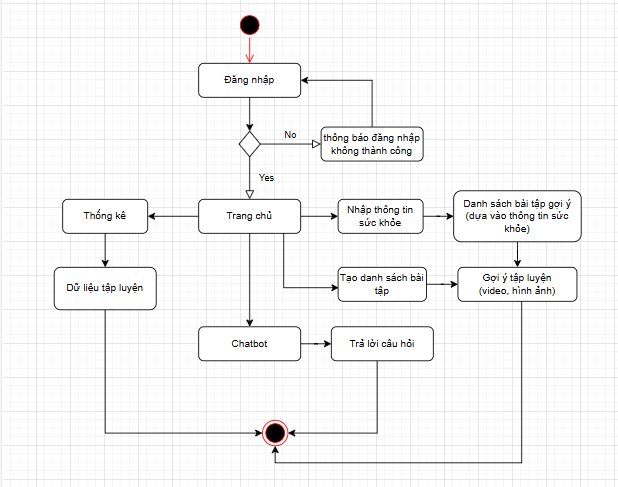
\includegraphics[width=0.86\textwidth,height=0.62\textheight,keepaspectratio]{tai_nguyen/media/image3.png}
    \caption{Luồng sử dụng tổng quan của website}
\end{figure}

\section{Kiến trúc tổng thể của hệ thống}

Hệ thống được chia thành bốn lớp: giao diện người dùng, route xử lý của Remix, cơ sở dữ liệu thông qua Prisma và các dịch vụ ngoài. Giao diện dùng React component và NextUI để tạo màn hình. Route Remix dùng loader để nạp dữ liệu ban đầu và action để xử lý dữ liệu gửi lên. Prisma đảm nhiệm truy vấn cơ sở dữ liệu. Auth0, chatbot và API video là các thành phần tích hợp ngoài.


Kiến trúc này phù hợp với đồ án vì một project có thể quản lý cả frontend và backend. Việc đặt logic trong các route giúp dễ trình bày mối liên hệ giữa màn hình, API và dữ liệu.


\begingroup
\setlength{\tabcolsep}{3pt}
\renewcommand{\arraystretch}{1.25}
\begin{longtable}{|P{0.220\textwidth}|P{0.330\textwidth}|P{0.370\textwidth}|}
\caption{Lớp kiến trúc và thành phần triển khai}\\
\hline
\textbf{Lớp} & \textbf{Thành phần} & \textbf{Vai trò} \\
\hline
\endfirsthead
\caption[]{Lớp kiến trúc và thành phần triển khai (tiếp theo)}\\
\hline
\textbf{Lớp} & \textbf{Thành phần} & \textbf{Vai trò} \\
\hline
\endhead
Giao diện & React, NextUI, Tailwind CSS, Recharts & Hiển thị form, bảng, thẻ bài tập, biểu đồ và chatbot. \\
\hline
Route Remix & loader, action, fetch API & Nạp dữ liệu, xử lý form và kết nối cơ sở dữ liệu. \\
\hline
Dữ liệu & Prisma, PostgreSQL & Lưu người dùng, bài tập, hồ sơ sức khỏe, kế hoạch và tiến trình. \\
\hline
Dịch vụ ngoài & Auth0, Dify/Coze, YouTube API & Xác thực, chatbot và video tham khảo bài tập. \\
\hline
\end{longtable}
\endgroup


\begin{figure}[H]
    \centering
    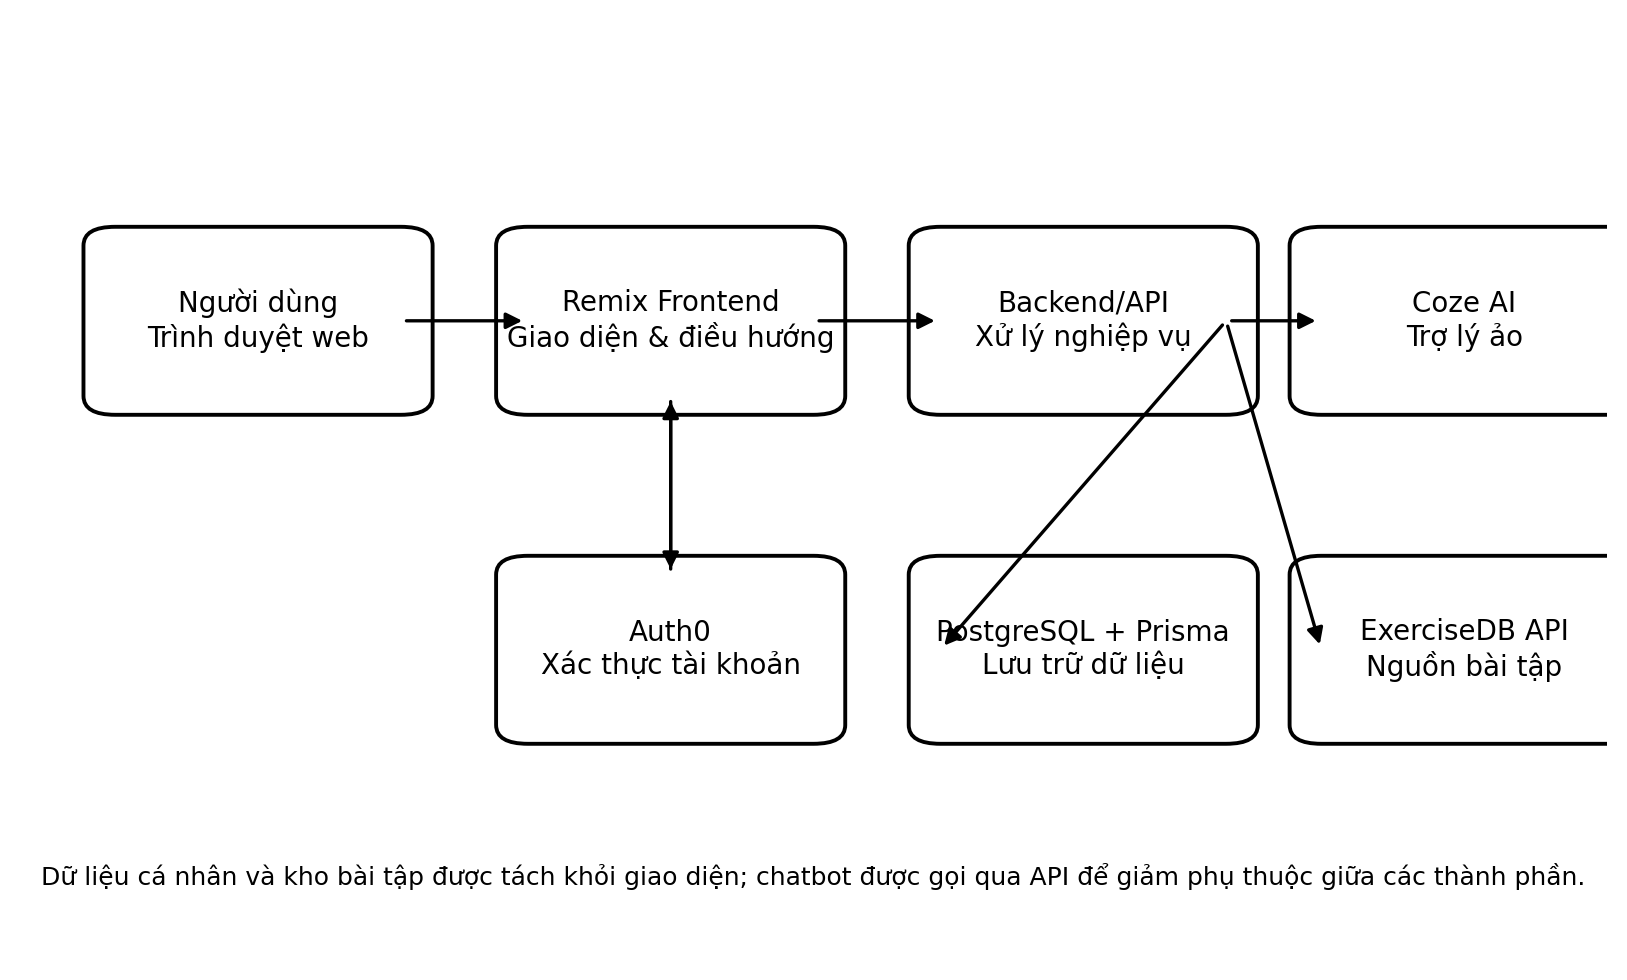
\includegraphics[width=0.86\textwidth,height=0.62\textheight,keepaspectratio]{tai_nguyen/media/image4.png}
    \caption{Kiến trúc logic của website tập luyện}
\end{figure}

\section{Tác nhân và phạm vi quyền}

\begingroup
\setlength{\tabcolsep}{3pt}
\renewcommand{\arraystretch}{1.25}
\begin{longtable}{|P{0.220\textwidth}|P{0.330\textwidth}|P{0.370\textwidth}|}
\caption{Tác nhân và quyền sử dụng}\\
\hline
\textbf{Tác nhân} & \textbf{Quyền chính} & \textbf{Giới hạn} \\
\hline
\endfirsthead
\caption[]{Tác nhân và quyền sử dụng (tiếp theo)}\\
\hline
\textbf{Tác nhân} & \textbf{Quyền chính} & \textbf{Giới hạn} \\
\hline
\endhead
User & Xem bài tập, cập nhật hồ sơ, nhận gợi ý, lập kế hoạch, lưu tiến trình, xem thống kê. & Chỉ thao tác dữ liệu của chính mình. \\
\hline
Admin & Xem dashboard, quản lý người dùng, quản lý bài tập. & Cần tài khoản có cờ isAdmin trong cơ sở dữ liệu. \\
\hline
Auth0 & Xác thực đăng nhập và trả hồ sơ người dùng. & Không xử lý dữ liệu tập luyện. \\
\hline
Chatbot & Trả lời câu hỏi hỗ trợ và hướng dẫn sử dụng. & Không đưa ra kết luận y tế hoặc phác đồ điều trị. \\
\hline
Prisma/Database & Lưu và truy xuất dữ liệu nghiệp vụ. & Không trực tiếp hiển thị giao diện. \\
\hline
\end{longtable}
\endgroup

\section{Đặc tả Use Case tổng quát}

Biểu đồ Use Case tổng quát mô tả mối quan hệ giữa người dùng, quản trị viên và các nhóm chức năng. User tương tác với các chức năng luyện tập, còn Admin chịu trách nhiệm vận hành dữ liệu và theo dõi tổng quan hệ thống.



\begin{figure}[H]
    \centering
    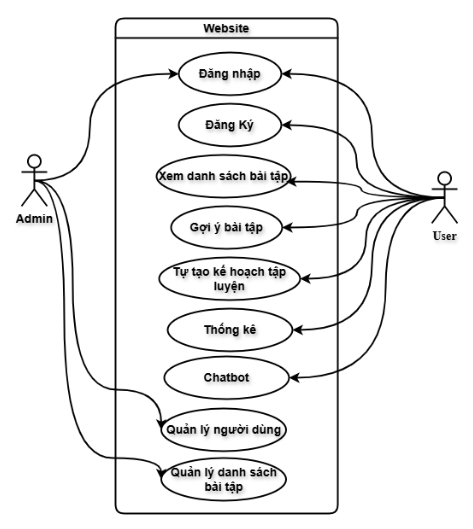
\includegraphics[width=0.86\textwidth,height=0.62\textheight,keepaspectratio]{tai_nguyen/media/image5.png}
    \caption{Use Case tổng thể của hệ thống}
\end{figure}

\begingroup
\setlength{\tabcolsep}{3pt}
\renewcommand{\arraystretch}{1.25}
\begin{longtable}{|P{0.220\textwidth}|P{0.330\textwidth}|P{0.370\textwidth}|}
\caption{Đặc tả Use Case chính}\\
\hline
\textbf{Mã} & \textbf{Tên Use Case} & \textbf{Kết quả mong đợi} \\
\hline
\endfirsthead
\caption[]{Đặc tả Use Case chính (tiếp theo)}\\
\hline
\textbf{Mã} & \textbf{Tên Use Case} & \textbf{Kết quả mong đợi} \\
\hline
\endhead
UC-01 & Đăng nhập & Người dùng được xác thực và chuyển vào hệ thống. \\
\hline
UC-02 & Cập nhật hồ sơ sức khỏe & Thông tin sức khỏe được lưu hoặc cập nhật thành công. \\
\hline
UC-03 & Xem danh sách bài tập & Danh sách bài tập được hiển thị, tìm kiếm và phân trang. \\
\hline
UC-04 & Nhận bài tập đề xuất & Danh sách bài tập phù hợp với hồ sơ được tạo và lưu tạm theo user. \\
\hline
UC-05 & Tạo kế hoạch tập & Các bài tập đã chọn được lưu vào WorkoutPlan. \\
\hline
UC-06 & Lưu tiến trình & Thời gian tập và trạng thái hoàn thành được ghi nhận. \\
\hline
UC-07 & Xem thống kê & Hệ thống tổng hợp dữ liệu 7 ngày, 30 ngày và phản hồi luyện tập. \\
\hline
UC-08 & Quản trị người dùng & Admin xem, sửa hoặc xóa tài khoản. \\
\hline
UC-09 & Quản trị bài tập & Admin thêm, sửa hoặc xóa dữ liệu bài tập. \\
\hline
\end{longtable}
\endgroup

\section{Thiết kế Use Case chi tiết}

Use Case chi tiết được phân rã để làm rõ phạm vi của từng nhóm chức năng. Việc phân rã giúp mỗi chức năng có đầu vào, thao tác và kết quả độc lập, thuận tiện cho kiểm thử về sau.



\begin{figure}[H]
    \centering
    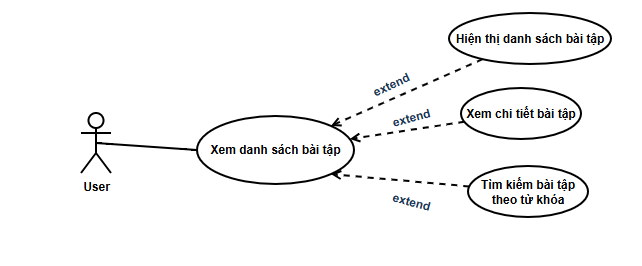
\includegraphics[width=0.86\textwidth,height=0.62\textheight,keepaspectratio]{tai_nguyen/media/image6.png}
    \caption{Use Case chi tiết cho nhóm xem bài tập}
\end{figure}

Use Case chi tiết được phân rã để làm rõ phạm vi của từng nhóm chức năng. Việc phân rã giúp mỗi chức năng có đầu vào, thao tác và kết quả độc lập, thuận tiện cho kiểm thử về sau.



\begin{figure}[H]
    \centering
    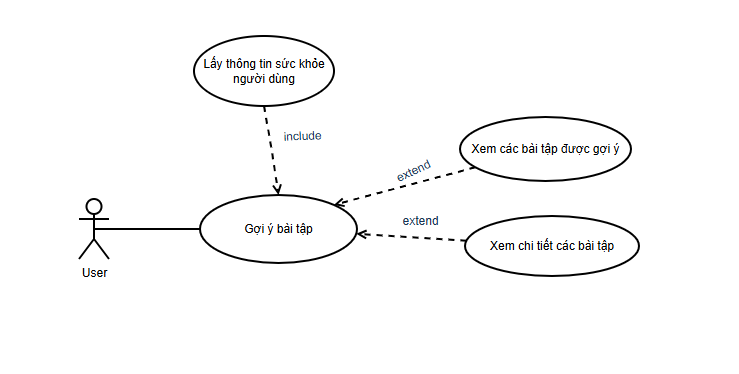
\includegraphics[width=0.86\textwidth,height=0.62\textheight,keepaspectratio]{tai_nguyen/media/image7.png}
    \caption{Use Case chi tiết cho nhóm đề xuất bài tập}
\end{figure}

Use Case chi tiết được phân rã để làm rõ phạm vi của từng nhóm chức năng. Việc phân rã giúp mỗi chức năng có đầu vào, thao tác và kết quả độc lập, thuận tiện cho kiểm thử về sau.



\begin{figure}[H]
    \centering
    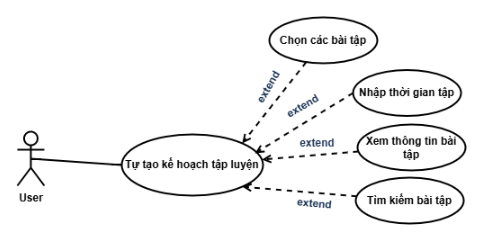
\includegraphics[width=0.86\textwidth,height=0.62\textheight,keepaspectratio]{tai_nguyen/media/image8.png}
    \caption{Use Case chi tiết cho nhóm lập kế hoạch tập}
\end{figure}

Use Case chi tiết được phân rã để làm rõ phạm vi của từng nhóm chức năng. Việc phân rã giúp mỗi chức năng có đầu vào, thao tác và kết quả độc lập, thuận tiện cho kiểm thử về sau.



\begin{figure}[H]
    \centering
    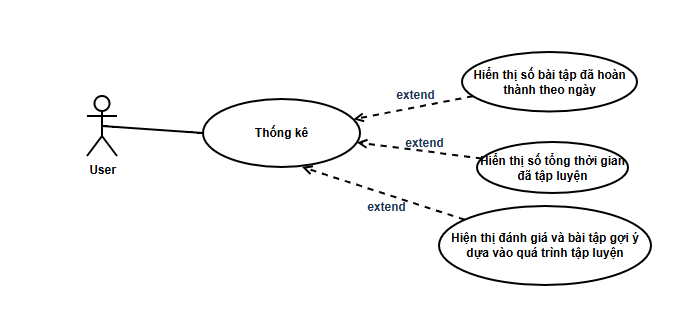
\includegraphics[width=0.86\textwidth,height=0.62\textheight,keepaspectratio]{tai_nguyen/media/image9.png}
    \caption{Use Case chi tiết cho nhóm thống kê tiến trình}
\end{figure}

Use Case chi tiết được phân rã để làm rõ phạm vi của từng nhóm chức năng. Việc phân rã giúp mỗi chức năng có đầu vào, thao tác và kết quả độc lập, thuận tiện cho kiểm thử về sau.



\begin{figure}[H]
    \centering
    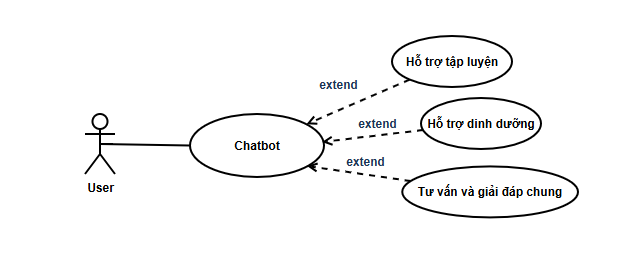
\includegraphics[width=0.86\textwidth,height=0.62\textheight,keepaspectratio]{tai_nguyen/media/image10.png}
    \caption{Use Case chi tiết cho nhóm chatbot}
\end{figure}

Use Case chi tiết được phân rã để làm rõ phạm vi của từng nhóm chức năng. Việc phân rã giúp mỗi chức năng có đầu vào, thao tác và kết quả độc lập, thuận tiện cho kiểm thử về sau.



\begin{figure}[H]
    \centering
    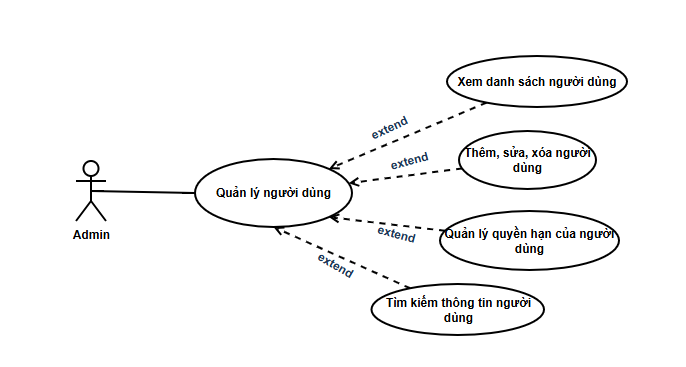
\includegraphics[width=0.86\textwidth,height=0.62\textheight,keepaspectratio]{tai_nguyen/media/image11.png}
    \caption{Use Case chi tiết cho quản trị người dùng}
\end{figure}

Use Case chi tiết được phân rã để làm rõ phạm vi của từng nhóm chức năng. Việc phân rã giúp mỗi chức năng có đầu vào, thao tác và kết quả độc lập, thuận tiện cho kiểm thử về sau.



\begin{figure}[H]
    \centering
    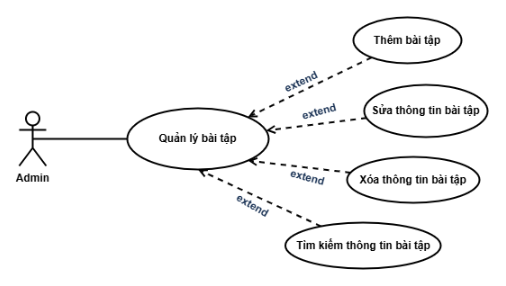
\includegraphics[width=0.86\textwidth,height=0.62\textheight,keepaspectratio]{tai_nguyen/media/image12.png}
    \caption{Use Case chi tiết cho quản trị bài tập}
\end{figure}

\section{Thiết kế chuỗi tương tác xử lý}

Biểu đồ trình tự giúp mô tả thứ tự trao đổi thông tin giữa người dùng, giao diện, route xử lý, cơ sở dữ liệu và dịch vụ ngoài. Các luồng quan trọng gồm đăng nhập, đăng ký, xem bài tập, nhận gợi ý, lưu kế hoạch, thống kê, chatbot và nhóm quản trị.



\begin{figure}[H]
    \centering
    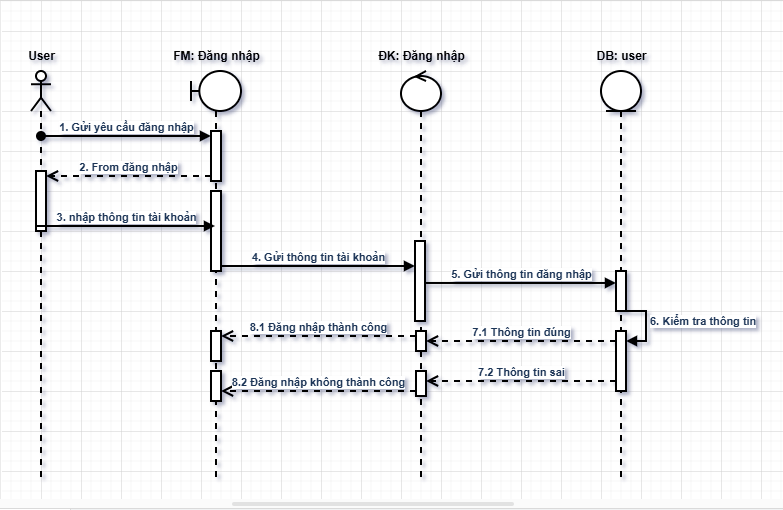
\includegraphics[width=0.86\textwidth,height=0.62\textheight,keepaspectratio]{tai_nguyen/media/image13.png}
    \caption{Trình tự xử lý đăng nhập}
\end{figure}


\begin{figure}[H]
    \centering
    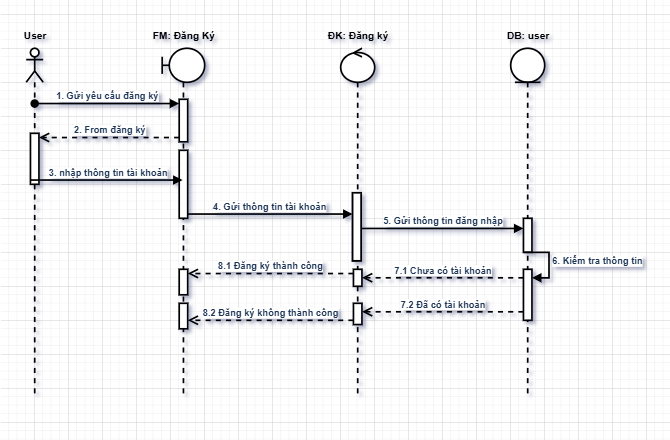
\includegraphics[width=0.86\textwidth,height=0.62\textheight,keepaspectratio]{tai_nguyen/media/image14.png}
    \caption{Trình tự xử lý đăng ký}
\end{figure}


\begin{figure}[H]
    \centering
    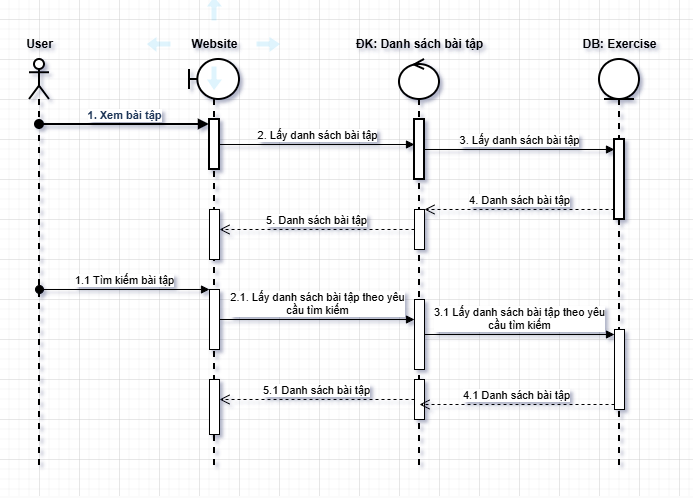
\includegraphics[width=0.86\textwidth,height=0.62\textheight,keepaspectratio]{tai_nguyen/media/image15.png}
    \caption{Trình tự xử lý khi xem thư viện bài tập}
\end{figure}


\begin{figure}[H]
    \centering
    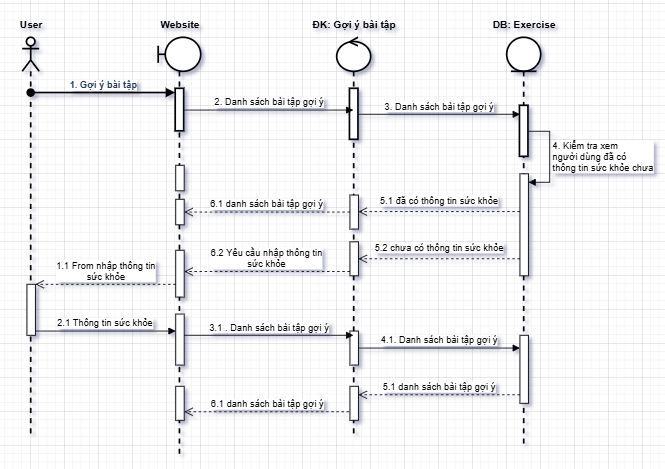
\includegraphics[width=0.86\textwidth,height=0.62\textheight,keepaspectratio]{tai_nguyen/media/image16.png}
    \caption{Trình tự xử lý khi đề xuất bài tập}
\end{figure}


\begin{figure}[H]
    \centering
    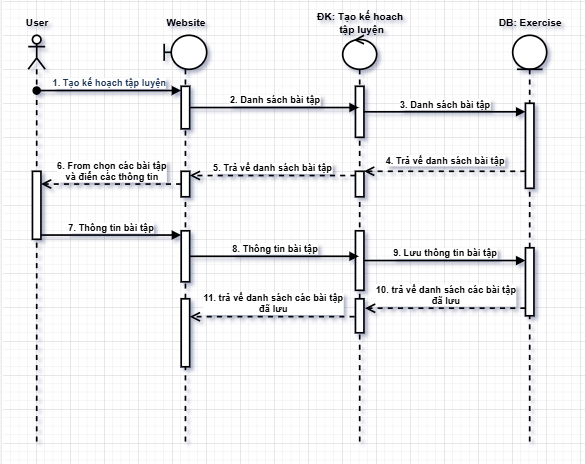
\includegraphics[width=0.86\textwidth,height=0.62\textheight,keepaspectratio]{tai_nguyen/media/image17.png}
    \caption{Trình tự xử lý khi tạo kế hoạch tập}
\end{figure}


\begin{figure}[H]
    \centering
    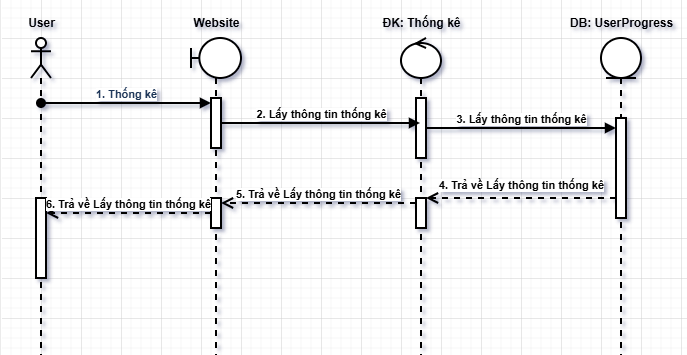
\includegraphics[width=0.86\textwidth,height=0.62\textheight,keepaspectratio]{tai_nguyen/media/image18.png}
    \caption{Trình tự xử lý khi tổng hợp thống kê}
\end{figure}


\begin{figure}[H]
    \centering
    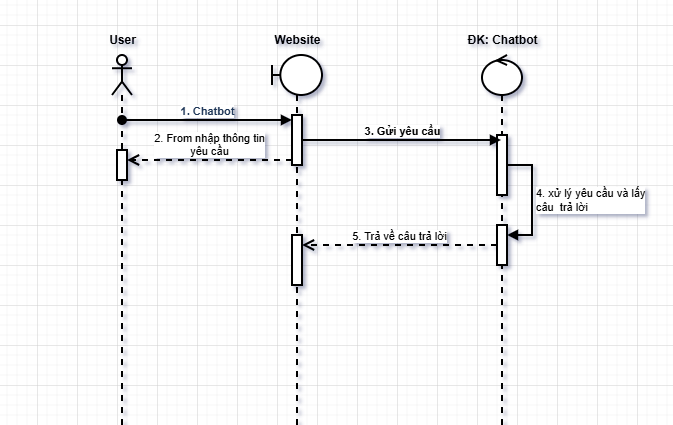
\includegraphics[width=0.86\textwidth,height=0.62\textheight,keepaspectratio]{tai_nguyen/media/image19.png}
    \caption{Trình tự xử lý khi người dùng hỏi chatbot}
\end{figure}


\begin{figure}[H]
    \centering
    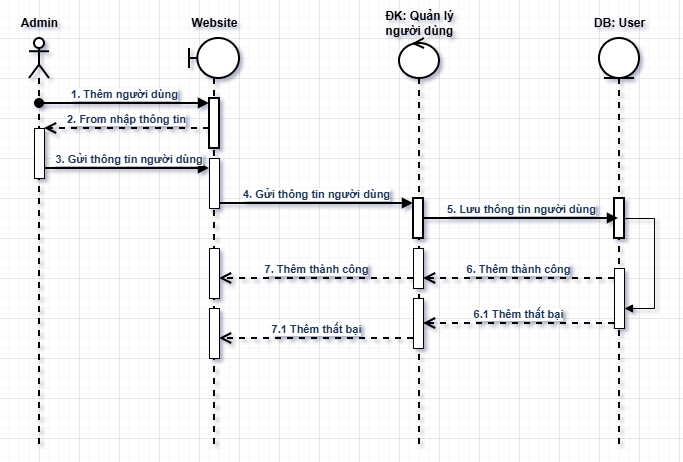
\includegraphics[width=0.86\textwidth,height=0.62\textheight,keepaspectratio]{tai_nguyen/media/image20.png}
    \caption{Trình tự xử lý khi thêm người dùng}
\end{figure}


\begin{figure}[H]
    \centering
    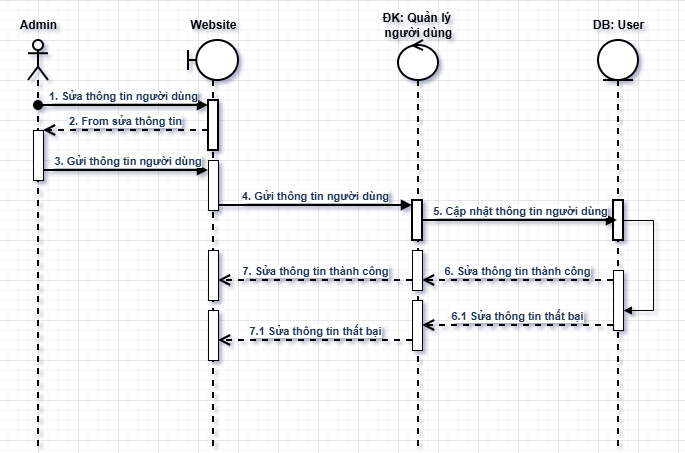
\includegraphics[width=0.86\textwidth,height=0.62\textheight,keepaspectratio]{tai_nguyen/media/image21.png}
    \caption{Trình tự xử lý khi cập nhật người dùng}
\end{figure}


\begin{figure}[H]
    \centering
    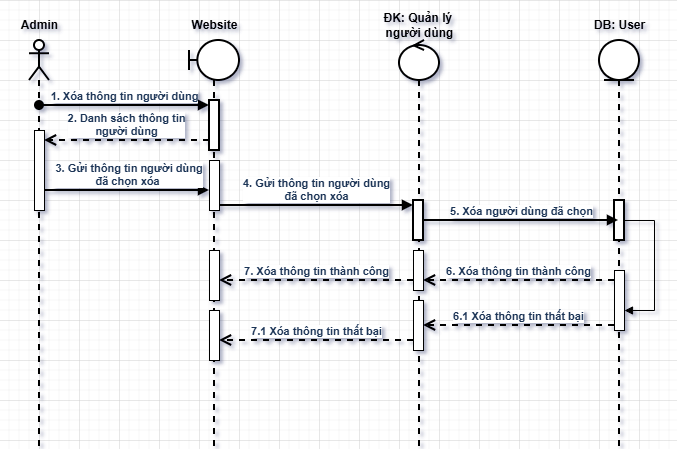
\includegraphics[width=0.86\textwidth,height=0.62\textheight,keepaspectratio]{tai_nguyen/media/image22.png}
    \caption{Trình tự xử lý khi xóa người dùng}
\end{figure}


\begin{figure}[H]
    \centering
    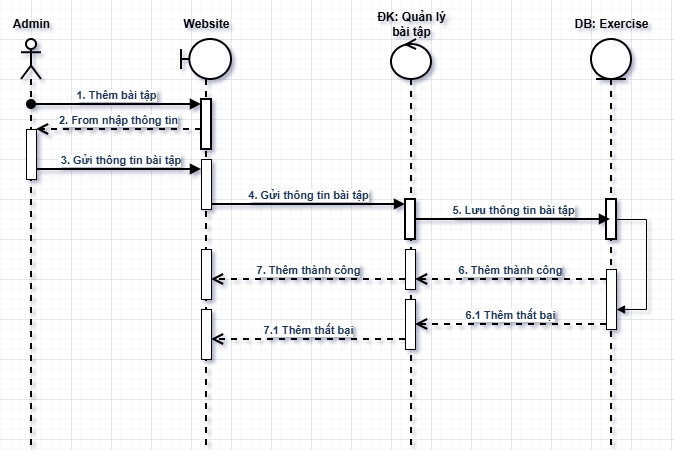
\includegraphics[width=0.86\textwidth,height=0.62\textheight,keepaspectratio]{tai_nguyen/media/image23.png}
    \caption{Trình tự xử lý khi thêm bài tập}
\end{figure}


\begin{figure}[H]
    \centering
    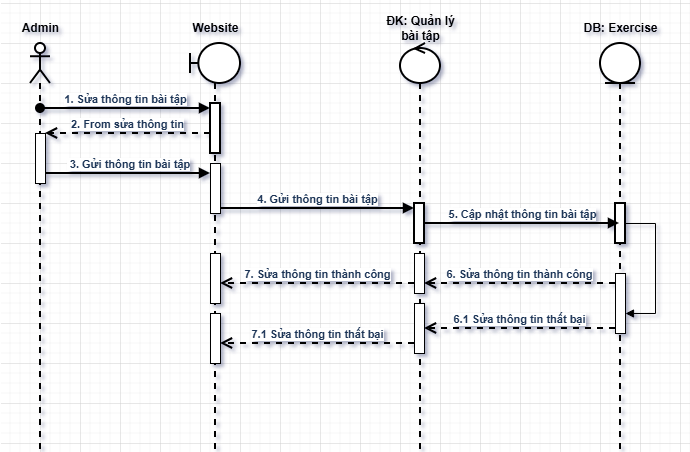
\includegraphics[width=0.86\textwidth,height=0.62\textheight,keepaspectratio]{tai_nguyen/media/image24.png}
    \caption{Trình tự xử lý khi cập nhật bài tập}
\end{figure}


\begin{figure}[H]
    \centering
    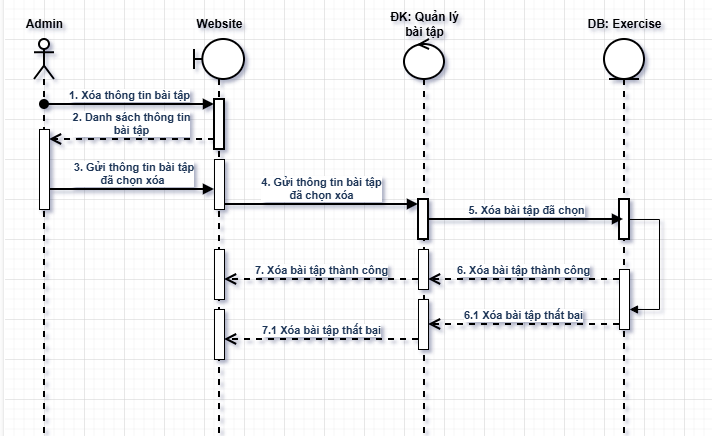
\includegraphics[width=0.86\textwidth,height=0.62\textheight,keepaspectratio]{tai_nguyen/media/image25.png}
    \caption{Trình tự xử lý khi xóa bài tập}
\end{figure}

\section{Thiết kế mô hình dữ liệu}

Mô hình dữ liệu của hệ thống được xây dựng quanh các thực thể chính: User, HealthStatus, Exercise, Workout, WorkoutPlan và UserProgress. User là trung tâm của dữ liệu cá nhân. HealthStatus lưu hồ sơ sức khỏe. Exercise lưu thư viện bài tập. Workout lưu danh sách bài tập đề xuất hoặc bài tập theo người dùng. WorkoutPlan lưu kế hoạch theo ngày. UserProgress ghi nhận tiến trình hoàn thành.


Các quan hệ này giúp hệ thống trả lời được những câu hỏi nghiệp vụ: người dùng hiện có hồ sơ sức khỏe nào, bài tập nào phù hợp, lịch tập đã lưu là gì, bài nào đã hoàn thành và kết quả thống kê trong giai đoạn gần đây ra sao.



\begin{figure}[H]
    \centering
    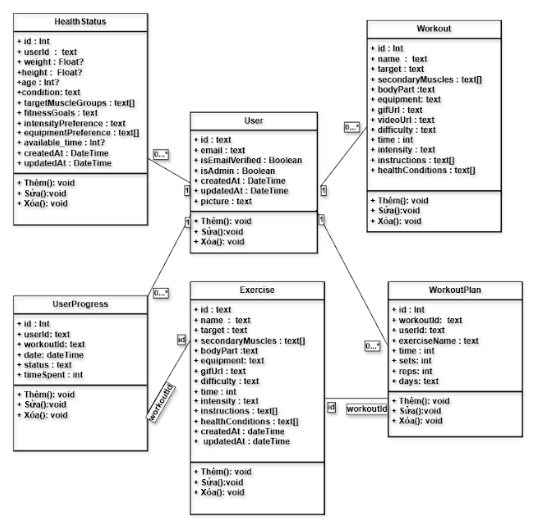
\includegraphics[width=0.86\textwidth,height=0.62\textheight,keepaspectratio]{tai_nguyen/media/image26.png}
    \caption{Mô hình lớp dữ liệu của hệ thống}
\end{figure}

\begingroup
\setlength{\tabcolsep}{3pt}
\renewcommand{\arraystretch}{1.25}
\begin{longtable}{|P{0.220\textwidth}|P{0.330\textwidth}|P{0.370\textwidth}|}
\caption{Mô tả các bảng dữ liệu chính}\\
\hline
\textbf{Bảng/Model} & \textbf{Trường tiêu biểu} & \textbf{Mục đích} \\
\hline
\endfirsthead
\caption[]{Mô tả các bảng dữ liệu chính (tiếp theo)}\\
\hline
\textbf{Bảng/Model} & \textbf{Trường tiêu biểu} & \textbf{Mục đích} \\
\hline
\endhead
User & id, email, userName, picture, isAdmin, isEmailVerified & Quản lý tài khoản và quyền truy cập. \\
\hline
HealthStatus & userId, weight, height, condition, fitnessGoals, intensityPreference & Lưu hồ sơ sức khỏe phục vụ cá nhân hóa. \\
\hline
Exercise & id, name, target, equipment, gifUrl, difficulty, intensity, time & Lưu kho bài tập và thuộc tính lọc. \\
\hline
Workout & userId, exercise fields & Lưu danh sách bài tập được gợi ý cho từng người dùng. \\
\hline
WorkoutPlan & userId, workoutId, date, time, sets, reps & Lưu kế hoạch luyện tập cá nhân. \\
\hline
UserProgress & userId, workoutId, timeSpent, status, date & Ghi nhận tiến trình hoàn thành bài tập. \\
\hline
Message & userId, sender, message & Lưu nội dung hội thoại nếu dùng route chatbotapi. \\
\hline
\end{longtable}
\endgroup

\section{Thiết kế route và API logic}

Trong Remix, route vừa là đường dẫn giao diện vừa có thể là endpoint xử lý dữ liệu. Thiết kế route của hệ thống được chia theo nhóm: xác thực, hồ sơ sức khỏe, bài tập, kế hoạch, tiến trình, thống kê, chatbot và quản trị.


\begingroup
\setlength{\tabcolsep}{3pt}
\renewcommand{\arraystretch}{1.25}
\begin{longtable}{|P{0.220\textwidth}|P{0.330\textwidth}|P{0.370\textwidth}|}
\caption{Ma trận route và chức năng}\\
\hline
\textbf{Route/File} & \textbf{Loại xử lý} & \textbf{Vai trò} \\
\hline
\endfirsthead
\caption[]{Ma trận route và chức năng (tiếp theo)}\\
\hline
\textbf{Route/File} & \textbf{Loại xử lý} & \textbf{Vai trò} \\
\hline
\endhead
auth.auth0.jsx, homeCallback.jsx & loader/action & Điều hướng xác thực Auth0 và nhận callback sau đăng nhập. \\
\hline
login.jsx & loader & Tạo người dùng nếu chưa có và nạp dữ liệu bài tập ban đầu. \\
\hline
home.jsx & loader + giao diện & Hiển thị thư viện bài tập, tìm kiếm và phân trang. \\
\hline
HealthStatus.jsx, healthstatusapi.jsx & loader/action & Nhập, lưu và cập nhật hồ sơ sức khỏe. \\
\hline
equipmentapi.jsx, musclesapi.jsx & loader & Trả danh sách thiết bị và nhóm cơ theo lựa chọn sức khỏe. \\
\hline
Recommended.workout.jsx & loader & Lọc bài tập theo hồ sơ và lưu danh sách gợi ý. \\
\hline
WorkoutPlan.jsx, Workoutplanapi.jsx & loader/action & Chọn bài tập và lưu kế hoạch tập luyện. \\
\hline
Workout.jsx, editworkoutapi.jsx, deleteapi.jsx & loader/action & Xem, sửa và xóa bài tập trong kế hoạch. \\
\hline
ExerciseDetail.jsx, userprogressapi.jsx & loader/action & Xem chi tiết, bật timer và lưu tiến trình. \\
\hline
Stats.jsx & loader + giao diện & Tổng hợp thống kê và phản hồi cá nhân hóa. \\
\hline
admin.jsx & loader + giao diện & Dashboard quản trị, CRUD user và bài tập. \\
\hline
chatbotapi2.jsx & component & Nhúng chatbot vào giao diện website. \\
\hline
\end{longtable}
\endgroup

\section{Thiết kế xử lý bảo mật và phân quyền}

Bảo mật trong hệ thống được triển khai ở nhiều mức. Mức đầu tiên là xác thực qua Auth0. Mức thứ hai là session cookie lưu userId để backend biết người dùng hiện tại. Mức thứ ba là kiểm tra quyền admin trước khi truy cập trang quản trị hoặc thực hiện thao tác quản lý.


Về nguyên tắc, không nên chỉ ẩn nút quản trị ở giao diện. Backend vẫn phải kiểm tra quyền trước khi cho phép sửa hoặc xóa dữ liệu. Điều này đặc biệt quan trọng với các action như update\_user, delete\_user, create\_exercise và delete\_exercise.


Các khóa API, token chatbot, secret session và khóa dịch vụ không nên ghi trực tiếp trong mã nguồn khi triển khai thật. Trong báo cáo, các giá trị cụ thể được lược bỏ hoặc chỉ mô tả vai trò để tránh lộ thông tin nhạy cảm.


\section{Thiết kế giao diện}

Giao diện người dùng được tổ chức theo các màn hình chính: trang giới thiệu, đăng nhập, trang chủ, hồ sơ sức khỏe, bài tập đề xuất, lập kế hoạch, lịch tập, thống kê, chi tiết bài tập và chatbot. Các màn hình dùng navbar và avatar để tạo lối điều hướng thống nhất.


Giao diện quản trị được thiết kế theo tab gồm dashboard, quản lý người dùng và quản lý bài tập. Cách tổ chức này giúp admin không bị lẫn giữa dữ liệu người dùng cuối và dữ liệu bài tập.


\section{Thiết kế thông báo và xử lý lỗi}

Hệ thống cần phản hồi rõ khi người dùng nhập thiếu dữ liệu, chưa có hồ sơ sức khỏe, chưa đăng nhập hoặc thao tác lưu thất bại. Trong mã nguồn, các route thường trả json kèm status 400, 401, 404 hoặc 500 tùy lỗi. Giao diện sử dụng toast để thông báo kết quả thao tác.


Đối với dữ liệu luyện tập, các trường như timeSpent, workoutId, status, sets và reps cần kiểm tra trước khi lưu. Với userprogressapi, nếu thiếu userId, workoutId hoặc timeSpent không hợp lệ, hệ thống trả lỗi thay vì ghi dữ liệu sai vào cơ sở dữ liệu.


	\chapter{TRIỂN KHAI}

\section{Môi trường triển khai và cấu trúc mã nguồn}

Mã nguồn được tổ chức theo cấu trúc của Remix. Thư mục app chứa root, entry.client, entry.server, các route giao diện, route xử lý API, server auth và server database. Cấu trúc này cho phép trình bày rõ từng phần triển khai theo chức năng nghiệp vụ thay vì chỉ mô tả công nghệ chung.


File root.jsx thiết lập Layout, NextUIProvider, import CSS, cấu hình font, nạp Google Translate và nhúng chatbot toàn cục. entry.client.jsx thực hiện hydrate giao diện trên trình duyệt; entry.server.jsx xử lý render phía server. db.server.js khởi tạo PrismaClient; auth.server.js cấu hình session và Auth0Strategy.


\begingroup
\setlength{\tabcolsep}{3pt}
\renewcommand{\arraystretch}{1.25}
\begin{longtable}{|P{0.220\textwidth}|P{0.330\textwidth}|P{0.370\textwidth}|}
\caption{Nhóm file nền tảng của project}\\
\hline
\textbf{File} & \textbf{Vai trò triển khai} & \textbf{Ghi chú} \\
\hline
\endfirsthead
\caption[]{Nhóm file nền tảng của project (tiếp theo)}\\
\hline
\textbf{File} & \textbf{Vai trò triển khai} & \textbf{Ghi chú} \\
\hline
\endhead
root.jsx & Khung layout, provider, CSS và chatbot toàn cục. & Có tích hợp nút dịch ngôn ngữ và component chatbot. \\
\hline
entry.client.jsx & Hydrate RemixBrowser phía client. & Dùng hydrateRoot và StrictMode. \\
\hline
entry.server.jsx & Render HTML phía server. & Dùng renderToPipeableStream, phân biệt bot và browser. \\
\hline
db.server.js & Khởi tạo PrismaClient. & Dùng singleton trong môi trường development. \\
\hline
auth.server.js & Cấu hình cookie session và Auth0. & Cần chuyển secret/callback theo môi trường khi deploy. \\
\hline
\end{longtable}
\endgroup

\section{Thu nhận và xử lý dữ liệu bài tập}

Dữ liệu bài tập được đưa vào hệ thống thông qua quá trình nạp và chuẩn hóa. Các file login.jsx, loader.jsx và saveExercises.jsx cho thấy hệ thống có cơ chế lưu bài tập vào cơ sở dữ liệu bằng Prisma upsert, đồng thời bổ sung các trường tính toán như độ khó, thời lượng, cường độ và nhóm sức khỏe phù hợp.


Việc bổ sung các trường này là cần thiết vì dữ liệu thô thường chưa đủ để phục vụ cá nhân hóa. Nếu một bài tập chỉ có tên và mô tả, hệ thống không thể lọc theo thể trạng hoặc thiết bị. Sau khi xử lý, mỗi bài tập có thể tham gia vào các truy vấn gợi ý và thống kê.



\begin{figure}[H]
    \centering
    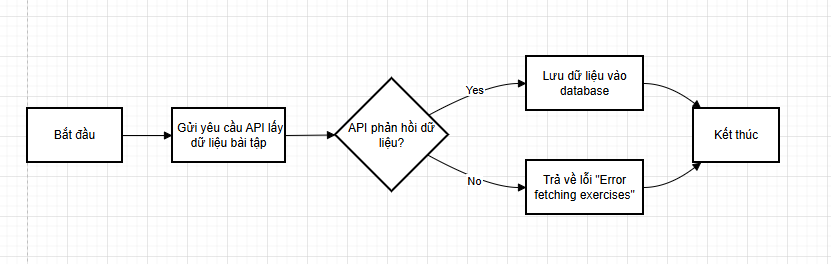
\includegraphics[width=0.86\textwidth,height=0.62\textheight,keepaspectratio]{tai_nguyen/media/image27.png}
    \caption{Quy trình thu nhận dữ liệu bài tập}
\end{figure}

\subsection{Xác định độ khó bài tập}

Hàm calculateDifficulty phân loại bài tập dựa trên thiết bị và bộ phận cơ thể. Các thiết bị nặng như barbell, kettlebell, smith machine hoặc trap bar thường được xếp mức hard. Thiết bị trung bình như dumbbell, resistance band, medicine ball hoặc stability ball được xếp medium. Các bài body weight hoặc thiết bị nhẹ có thể được xếp easy. Nếu thiết bị chưa đủ căn cứ, hệ thống xét tiếp bodyPart để điều chỉnh.



\begin{figure}[H]
    \centering
    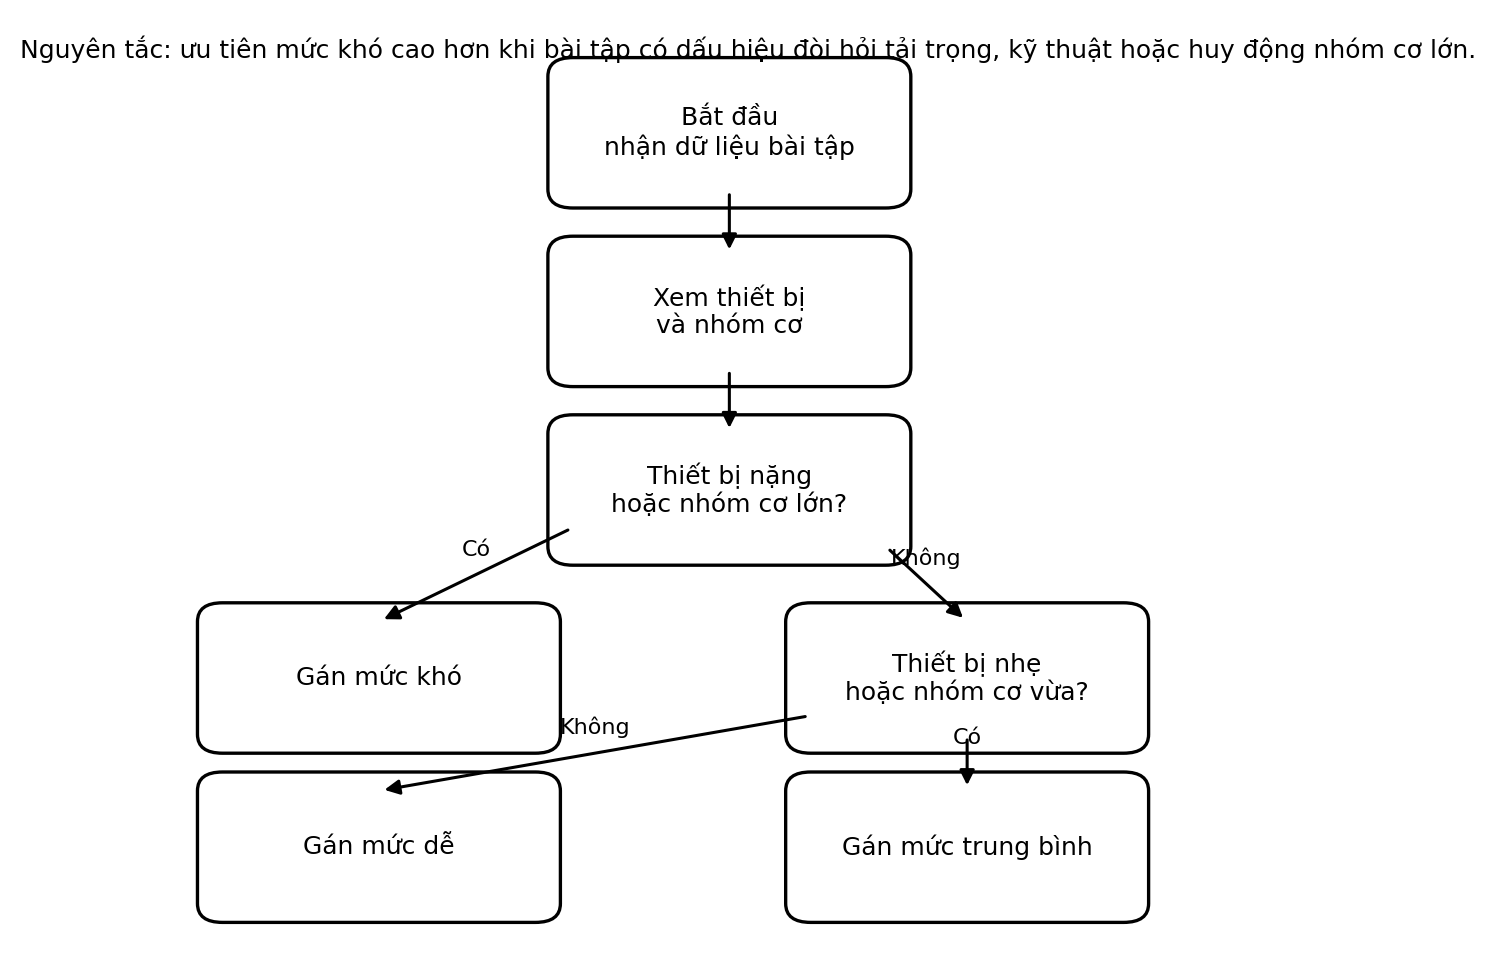
\includegraphics[width=0.86\textwidth,height=0.62\textheight,keepaspectratio]{tai_nguyen/media/image28.png}
    \caption{Quy tắc xác định độ khó bài tập}
\end{figure}

\subsection{Ước lượng thời lượng bài tập}

Hàm calculateTime bắt đầu từ thời gian cơ bản, sau đó cộng hoặc trừ theo thiết bị, nhóm cơ và độ khó. Bài tập dùng thiết bị nặng, tác động nhóm cơ lớn hoặc có độ khó cao sẽ có thời lượng ước lượng lớn hơn. Cách tính này không thay thế giáo án chuyên nghiệp nhưng đủ để hệ thống có trường time phục vụ lọc và hiển thị.



\begin{figure}[H]
    \centering
    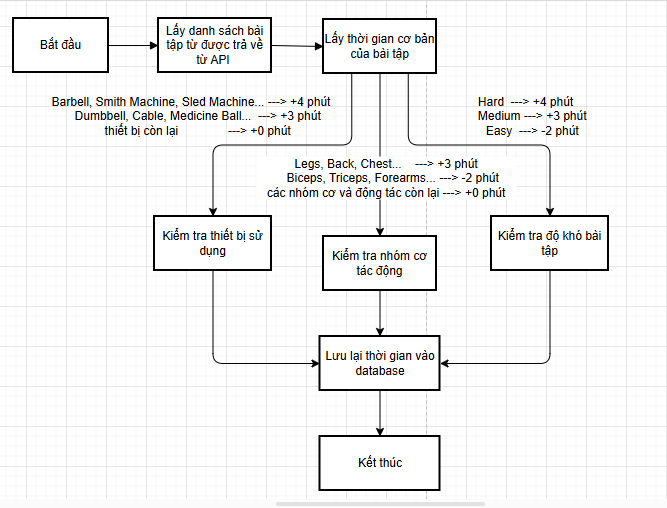
\includegraphics[width=0.86\textwidth,height=0.62\textheight,keepaspectratio]{tai_nguyen/media/image29.png}
    \caption{Quy tắc ước lượng thời lượng bài tập}
\end{figure}

\subsection{Phân loại cường độ}

Hàm calculateIntensity ánh xạ bài tập thành ba mức low, moderate và high. Những bài dùng thiết bị nặng hoặc tác động nhóm cơ lớn thường được xếp high; bài dùng dumbbell, cable, medicine ball hoặc tác động vai, tay được xếp moderate; các trường hợp còn lại mặc định low. Trường intensity là điều kiện quan trọng khi người dùng chọn cường độ mong muốn.



\begin{figure}[H]
    \centering
    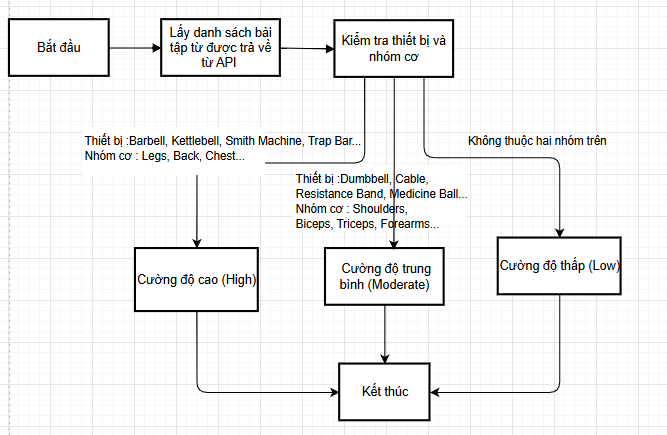
\includegraphics[width=0.86\textwidth,height=0.62\textheight,keepaspectratio]{tai_nguyen/media/image30.png}
    \caption{Quy tắc phân loại cường độ vận động}
\end{figure}

\subsection{Ánh xạ tình trạng sức khỏe}

Hàm calculateHealthConditions gắn bài tập với nhóm sức khỏe. Bài cường độ cao chỉ phù hợp với very healthy; bài moderate phù hợp với normal health và very healthy; bài low có thể phù hợp với weak health, normal health và very healthy. Quy tắc này thể hiện nguyên tắc an toàn: người sức khỏe yếu không nên được gợi ý bài quá nặng.



\begin{figure}[H]
    \centering
    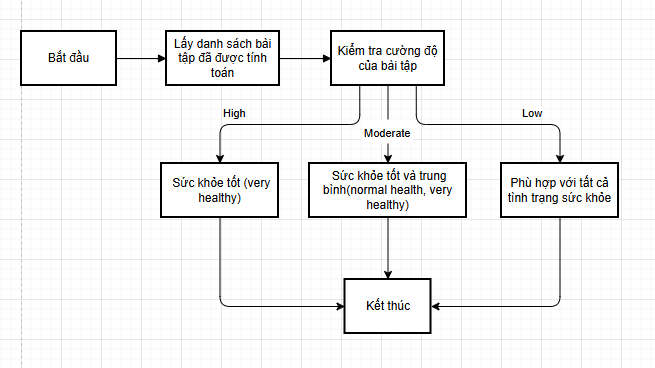
\includegraphics[width=0.86\textwidth,height=0.62\textheight,keepaspectratio]{tai_nguyen/media/image31.png}
    \caption{Quy tắc ánh xạ bài tập với nhóm sức khỏe}
\end{figure}

\section{Triển khai xác thực và quản lý phiên}

Xác thực được triển khai bằng Auth0. Khi người dùng chọn đăng nhập, route auth.auth0.jsx gọi authenticator.authenticate với chiến lược auth0. Sau callback, route homeCallback.jsx điều hướng người dùng về login.jsx. Tại login.jsx, hệ thống kiểm tra email trong cơ sở dữ liệu, tạo user mới nếu chưa có, sau đó lưu userId vào session.


Session được tạo bằng createCookieSessionStorage. Cookie đặt httpOnly để hạn chế truy cập từ JavaScript phía trình duyệt. Trong môi trường production, trường secure cần bật theo biến NODE\_ENV. Cách thiết kế này giúp các route xử lý dữ liệu đọc userId từ session thay vì phụ thuộc dữ liệu gửi từ client.


\section{Triển khai hồ sơ sức khỏe}

Trang HealthStatus.jsx cho phép người dùng nhập các trường sức khỏe và mục tiêu tập luyện. Loader của trang lấy người dùng hiện tại, đọc bản ghi HealthStatus nếu có, đồng thời chuẩn bị danh sách thiết bị và nhóm cơ ban đầu. Khi người dùng thay đổi cường độ, giao diện gọi equipmentapi để lấy danh sách thiết bị phù hợp. Khi chọn thiết bị, giao diện gọi musclesapi để lấy nhóm cơ tương ứng.


healthstatusapi.jsx xử lý lưu dữ liệu. Route này đọc formData, chuyển kiểu số cho cân nặng, chiều cao, tuổi, thời gian rảnh và dùng getUserIdFromSession để xác định chủ sở hữu. Nếu người dùng đã có hồ sơ, hệ thống update; nếu chưa có, hệ thống create. Cách xử lý này bảo đảm mỗi người dùng có thể cập nhật hồ sơ nhiều lần mà không tạo bản ghi trùng.


\section{Triển khai chức năng gợi ý bài tập}

Recommended.workout.jsx là route trọng tâm của chức năng cá nhân hóa. Hàm getRecommendedExercises đọc targetMuscleGroups, equipmentPreference, intensityPreference và condition từ HealthStatus. Sau đó hệ thống truy vấn Exercise với điều kiện AND, loại bỏ các điều kiện rỗng bằng filter(Boolean).


Sau khi nhận danh sách bài tập phù hợp, route xóa các bản ghi Workout cũ của người dùng và tạo danh sách mới. Việc làm mới danh sách giúp dữ liệu gợi ý luôn phản ánh hồ sơ sức khỏe hiện tại. Khi người dùng thay đổi cường độ, thiết bị hoặc nhóm cơ, kết quả gợi ý ở lần mở sau sẽ được tính lại.


\begingroup
\setlength{\tabcolsep}{3pt}
\renewcommand{\arraystretch}{1.25}
\begin{longtable}{|P{0.220\textwidth}|P{0.330\textwidth}|P{0.370\textwidth}|}
\caption{Điều kiện lọc trong chức năng gợi ý}\\
\hline
\textbf{Dữ liệu hồ sơ} & \textbf{Điều kiện truy vấn} & \textbf{Ý nghĩa} \\
\hline
\endfirsthead
\caption[]{Điều kiện lọc trong chức năng gợi ý (tiếp theo)}\\
\hline
\textbf{Dữ liệu hồ sơ} & \textbf{Điều kiện truy vấn} & \textbf{Ý nghĩa} \\
\hline
\endhead
targetMuscleGroups & target in danh sách nhóm cơ & Chỉ lấy bài tác động đúng nhóm cơ người dùng chọn. \\
\hline
equipmentPreference & equipment in danh sách thiết bị & Loại bỏ bài tập yêu cầu thiết bị người dùng không có. \\
\hline
intensityPreference & intensity bằng cường độ đã chọn & Giữ mức vận động phù hợp mong muốn. \\
\hline
condition & healthConditions hasSome condition & Chọn bài có nhóm sức khỏe tương thích. \\
\hline
\end{longtable}
\endgroup

\section{Triển khai lập kế hoạch và lịch tập}

WorkoutPlan.jsx hiển thị danh sách bài tập để người dùng lựa chọn và nhập thông tin kế hoạch như ngày tập, thời gian, số set và số rep. Khi người dùng lưu, dữ liệu selectedExercises được gửi đến Workoutplanapi.jsx.


Workoutplanapi.jsx đọc selectedExercises, lấy userId từ session, sau đó tạo từng bản ghi WorkoutPlan trong cơ sở dữ liệu. Trang Workout.jsx đọc danh sách kế hoạch của người dùng, include thông tin bài tập liên quan và hiển thị theo nhóm ngày. Người dùng có thể sửa thông số bằng editworkoutapi.jsx hoặc xóa kế hoạch bằng deleteapi.jsx.


\section{Triển khai chi tiết bài tập và ghi nhận tiến trình}

ExerciseDetail.jsx và ExerciseDetaill.jsx hiển thị thông tin chi tiết của bài tập, gồm nhóm cơ chính, nhóm cơ phụ, thiết bị, độ khó, ảnh động và hướng dẫn. Trang này có đồng hồ đếm thời gian để người dùng bắt đầu, tạm dừng, đặt lại và lưu thời gian tập.


Khi người dùng nhấn Save, giao diện gửi workoutId, timeSpent và status đến userprogressapi.jsx. Route này kiểm tra userId, kiểm tra bài tập và người dùng có tồn tại, sau đó update hoặc create bản ghi UserProgress. Nhờ vậy, cùng một bài tập có thể được cập nhật tiến trình thay vì tạo nhiều bản ghi không kiểm soát.


\section{Triển khai thống kê và phản hồi cá nhân hóa}

Stats.jsx tổng hợp dữ liệu tiến trình của người dùng và đánh giá theo giai đoạn. Route này đọc userProgress, healthStatus và danh sách bài tập, sau đó tạo các chỉ số phục vụ biểu đồ. Giao diện sử dụng BarChart, PieChart và các thành phần trực quan để người dùng dễ theo dõi.


Hàm generatePersonalizedFeedback tạo phản hồi theo kết quả weekly và monthly. Nếu hiệu suất cần cải thiện, hệ thống khuyến khích tập đều hơn và bắt đầu bằng phiên ngắn. Nếu hiệu suất trung bình, hệ thống gợi ý tăng dần cường độ. Nếu kết quả tốt, hệ thống khuyến khích duy trì và thử thách phù hợp. Ngoài ra, Stats.jsx còn có hàm getRecommendedExercises để đề xuất thêm bài tập dựa trên đánh giá mới.


\section{Triển khai chatbot hỗ trợ}

Chatbot được nhúng thông qua chatbotapi2.jsx. Component tạo cấu hình window.difyChatbotConfig, chèn script embed và thêm CSS để tùy biến nút bong bóng chat, biểu tượng, kích thước cửa sổ và khả năng responsive trên màn hình nhỏ.


Bên cạnh chatbot nhúng, mã nguồn còn có chatbotapi.jsx để lưu tin nhắn vào bảng message với userId, sender và message. Cách này có thể được dùng để mở rộng lịch sử hội thoại nội bộ nếu hệ thống muốn tự quản lý log chat thay vì chỉ dùng nền tảng chatbot bên ngoài.



\begin{figure}[H]
    \centering
    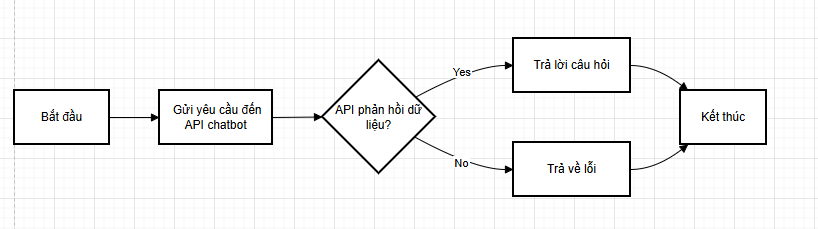
\includegraphics[width=0.86\textwidth,height=0.62\textheight,keepaspectratio]{tai_nguyen/media/image32.png}
    \caption{Luồng tích hợp chatbot vào website}
\end{figure}


\begin{figure}[H]
    \centering
    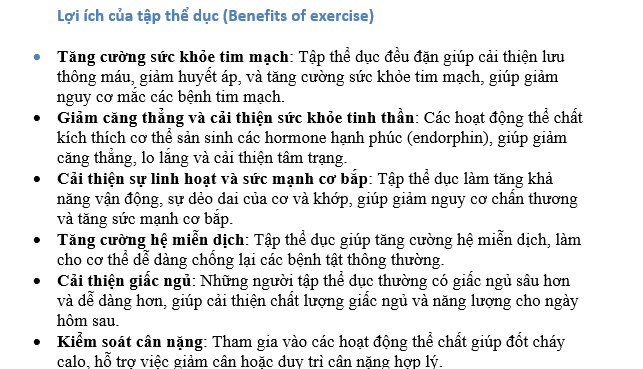
\includegraphics[width=0.86\textwidth,height=0.62\textheight,keepaspectratio]{tai_nguyen/media/image33.png}
    \caption{Bộ dữ liệu câu hỏi dùng cho chatbot}
\end{figure}


\begin{figure}[H]
    \centering
    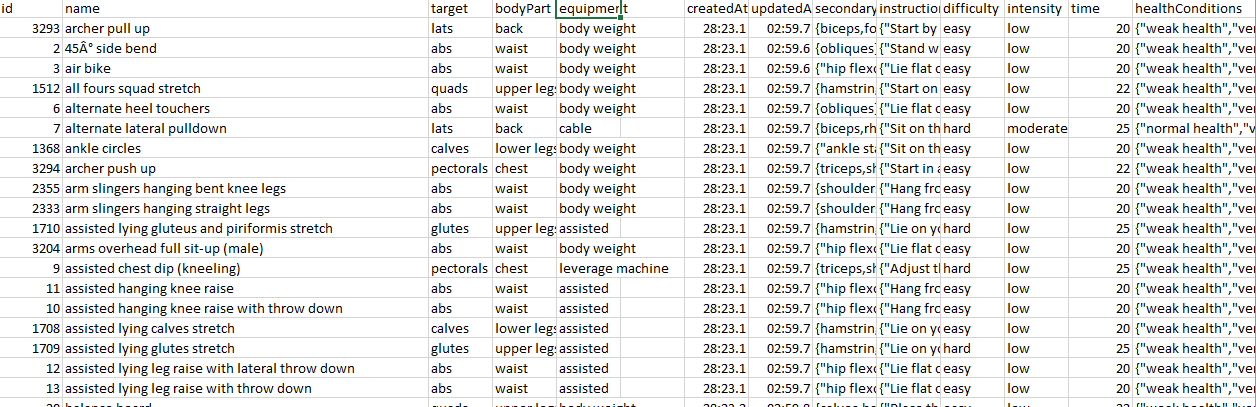
\includegraphics[width=0.86\textwidth,height=0.62\textheight,keepaspectratio]{tai_nguyen/media/image34.png}
    \caption{Bộ dữ liệu bài tập dùng cho chatbot}
\end{figure}


\begin{figure}[H]
    \centering
    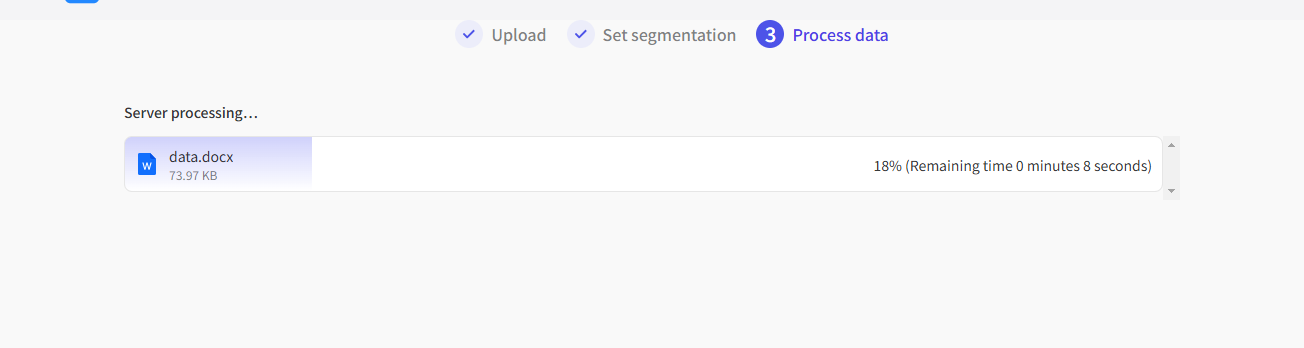
\includegraphics[width=0.86\textwidth,height=0.62\textheight,keepaspectratio]{tai_nguyen/media/image35.png}
    \caption{Quá trình nạp dữ liệu hỏi đáp cho chatbot}
\end{figure}


\begin{figure}[H]
    \centering
    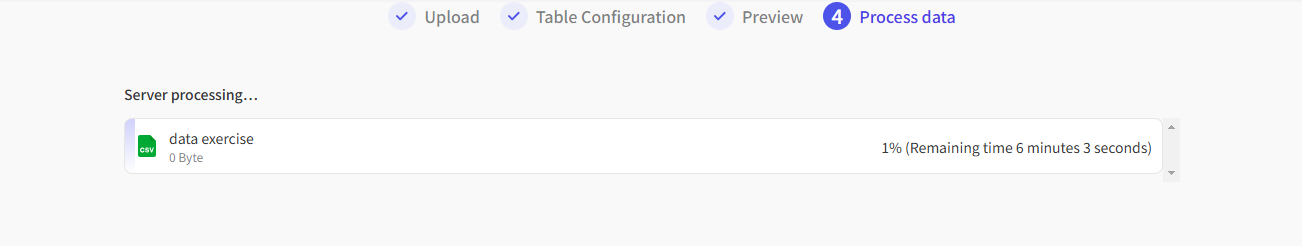
\includegraphics[width=0.86\textwidth,height=0.62\textheight,keepaspectratio]{tai_nguyen/media/image36.png}
    \caption{Quá trình nạp dữ liệu bài tập cho chatbot}
\end{figure}

\section{Triển khai giao diện người dùng}

Các giao diện chính được xây dựng theo luồng sử dụng của người dùng. Phần dưới đây mô tả vai trò của từng màn hình và minh chứng giao diện tương ứng.


Màn hình đăng nhập là điểm bắt đầu của người dùng đã có tài khoản. Từ đây, người dùng được chuyển sang Auth0 để xác thực. Nếu tài khoản hợp lệ, hệ thống điều hướng về trang sau đăng nhập và lưu phiên làm việc.



\begin{figure}[H]
    \centering
    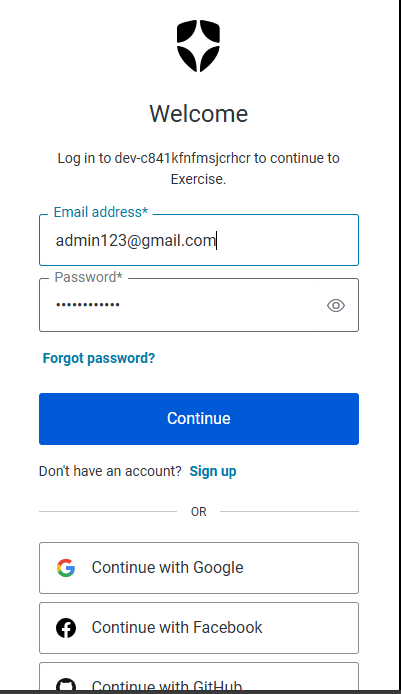
\includegraphics[width=0.86\textwidth,height=0.62\textheight,keepaspectratio]{tai_nguyen/media/image37.png}
    \caption{Giao diện đăng nhập tài khoản}
\end{figure}

Màn hình đăng ký phục vụ người dùng mới. Trong phiên bản dùng Auth0, quá trình tạo tài khoản có thể do Auth0 xử lý, còn website tiếp tục tạo bản ghi User trong cơ sở dữ liệu nội bộ khi đăng nhập thành công lần đầu.



\begin{figure}[H]
    \centering
    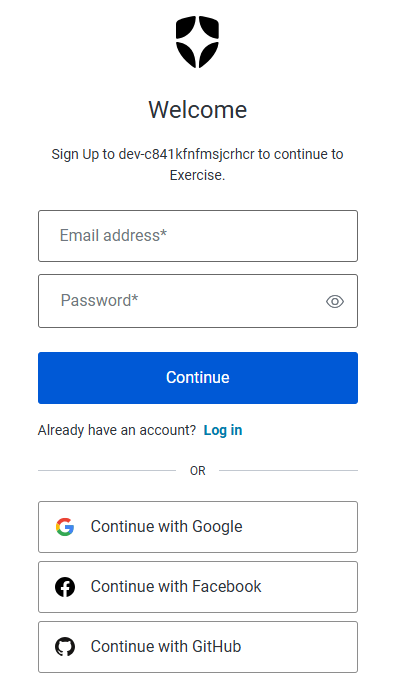
\includegraphics[width=0.86\textwidth,height=0.62\textheight,keepaspectratio]{tai_nguyen/media/image38.png}
    \caption{Giao diện tạo tài khoản mới}
\end{figure}

Trang chủ hiển thị thư viện bài tập, banner, các nhóm nội dung giới thiệu và thanh tìm kiếm. Danh sách bài tập được phân trang để giảm tải giao diện khi dữ liệu lớn.



\begin{figure}[H]
    \centering
    
\includegraphics[width=0.86\textwidth,height=0.62\textheight,keepaspectratio]{tai_nguyen/media/image39.png}
    \caption{Giao diện trang chủ sau khi đăng nhập}
\end{figure}

Trang chủ hiển thị thư viện bài tập, banner, các nhóm nội dung giới thiệu và thanh tìm kiếm. Danh sách bài tập được phân trang để giảm tải giao diện khi dữ liệu lớn.



\begin{figure}[H]
    \centering
    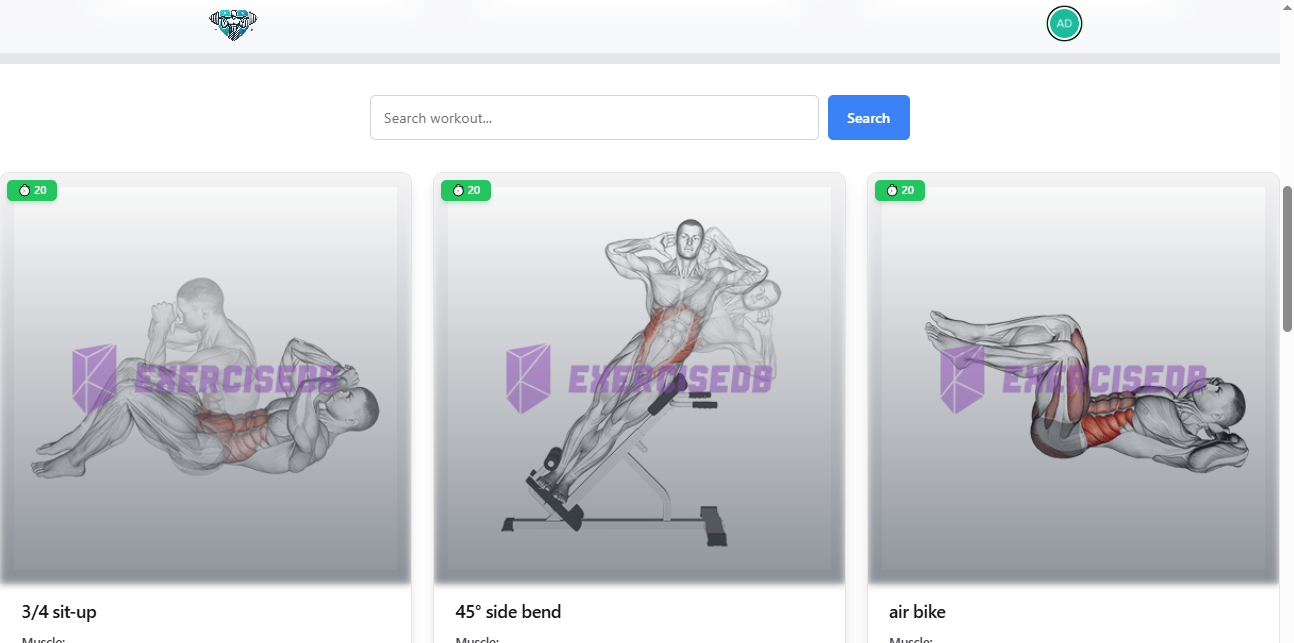
\includegraphics[width=0.86\textwidth,height=0.62\textheight,keepaspectratio]{tai_nguyen/media/image40.png}
    \caption{Bố cục nội dung trang chủ và danh sách bài tập}
\end{figure}

Trang hồ sơ sức khỏe là bước quan trọng trước khi nhận gợi ý. Người dùng khai báo tình trạng, mục tiêu, thiết bị, nhóm cơ và thời gian, từ đó hệ thống có dữ liệu để cá nhân hóa.



\begin{figure}[H]
    \centering
    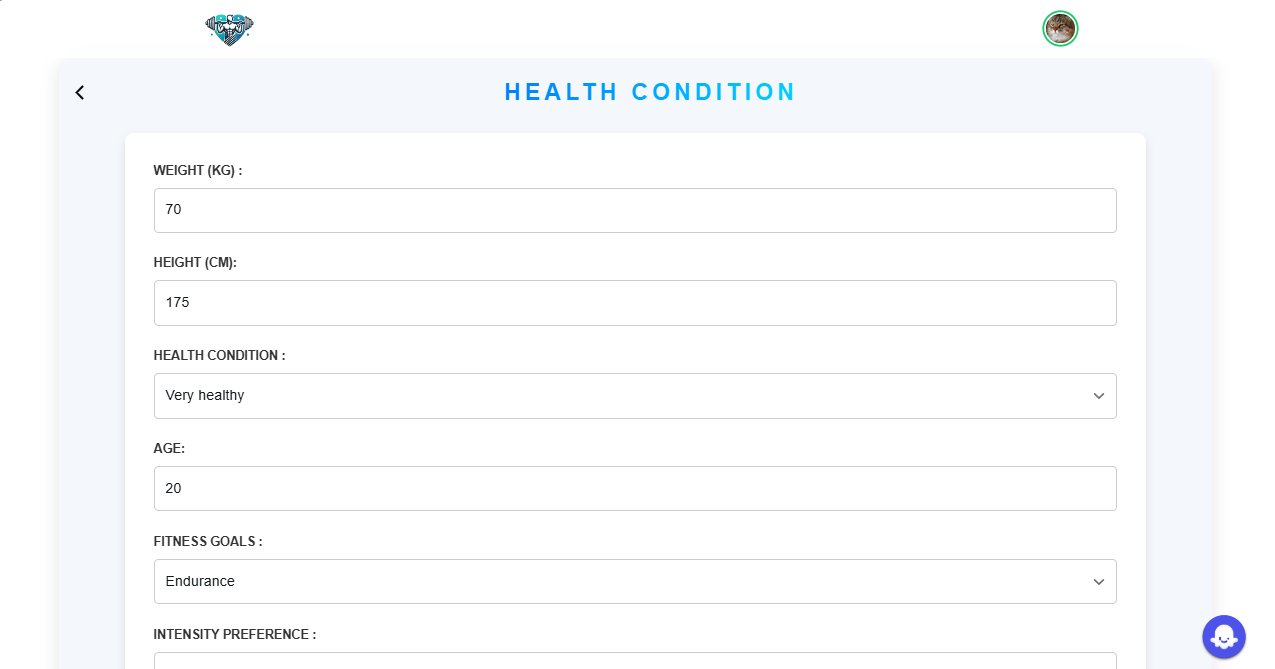
\includegraphics[width=0.86\textwidth,height=0.62\textheight,keepaspectratio]{tai_nguyen/media/image41.png}
    \caption{Giao diện cập nhật hồ sơ sức khỏe}
\end{figure}

Trang bài tập đề xuất hiển thị kết quả sau khi lọc theo hồ sơ sức khỏe. Người dùng có thể xem thông tin cơ bản, hình minh họa và chuyển sang các thao tác tiếp theo.



\begin{figure}[H]
    \centering
    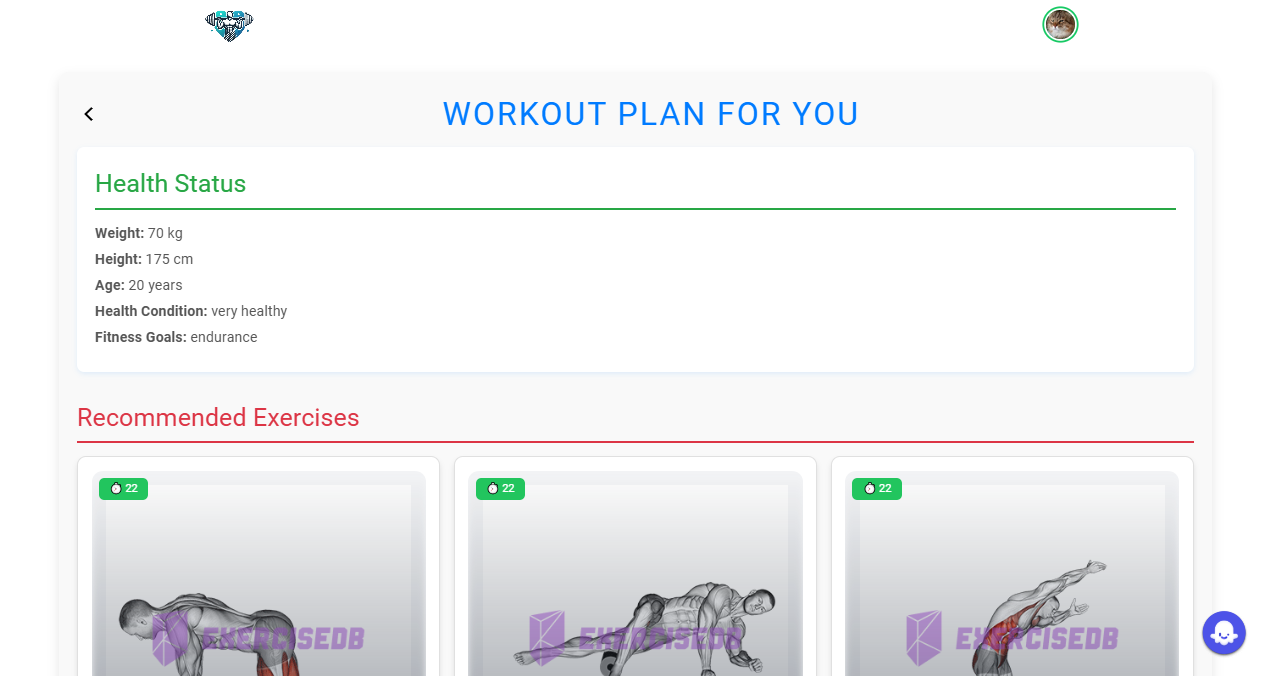
\includegraphics[width=0.86\textwidth,height=0.62\textheight,keepaspectratio]{tai_nguyen/media/image42.png}
    \caption{Giao diện danh sách bài tập đề xuất}
\end{figure}

Trang lập kế hoạch giúp người dùng chọn bài tập và đưa vào lịch cá nhân. Đây là bước chuyển từ gợi ý sang kế hoạch cụ thể có ngày, thời lượng, số hiệp và số lần lặp.



\begin{figure}[H]
    \centering
    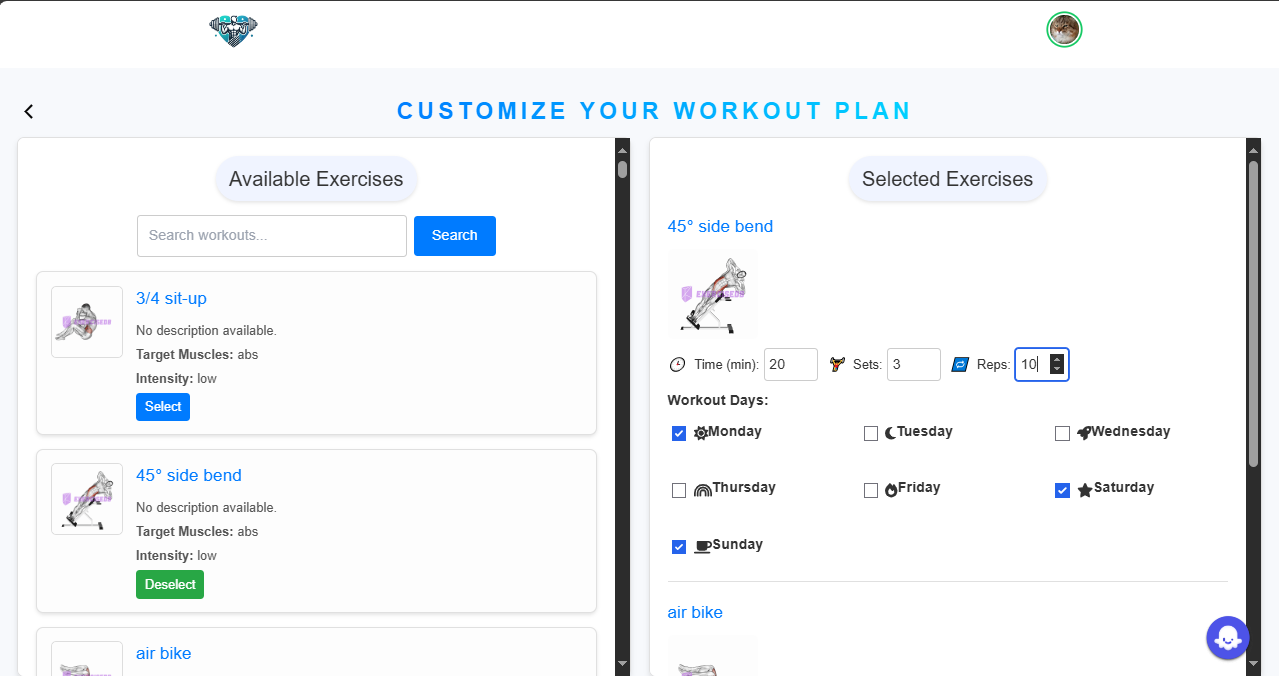
\includegraphics[width=0.86\textwidth,height=0.62\textheight,keepaspectratio]{tai_nguyen/media/image43.png}
    \caption{Giao diện lập kế hoạch tập luyện}
\end{figure}

Trang lịch bài tập cá nhân hiển thị các bài đã được lưu theo ngày. Người dùng có thể chỉnh sửa hoặc xóa bài tập trong kế hoạch nếu lịch thay đổi.



\begin{figure}[H]
    \centering
    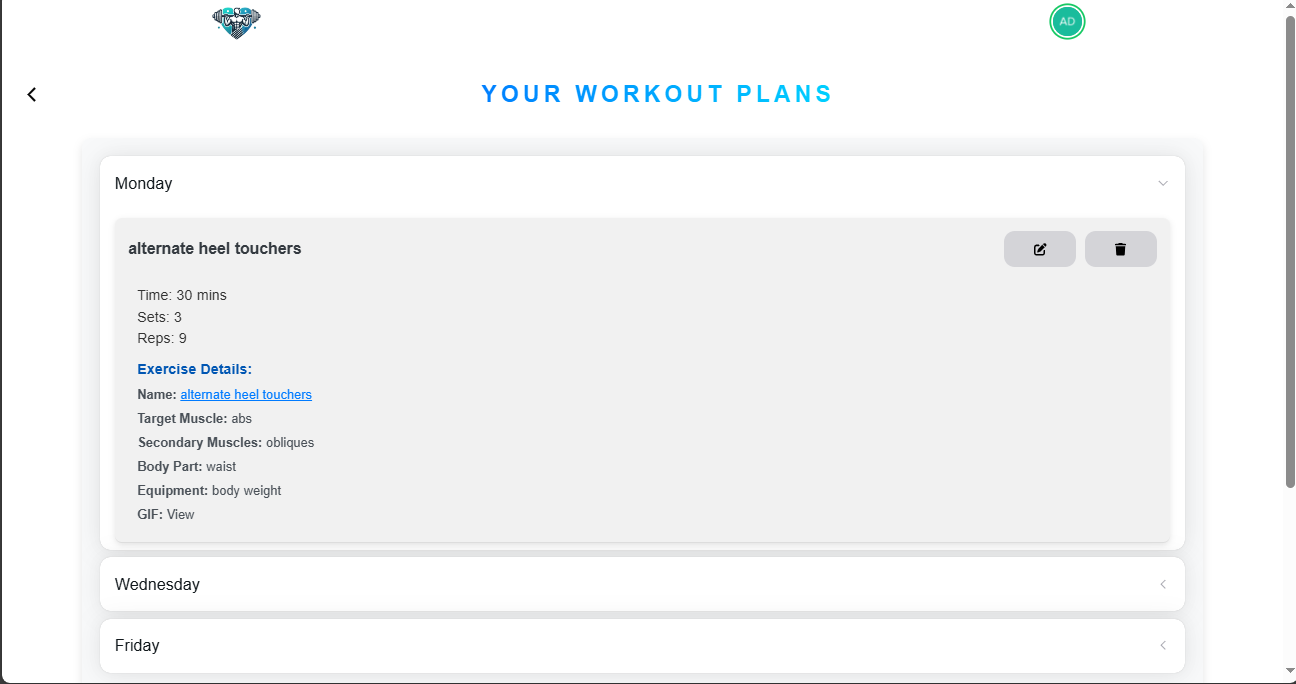
\includegraphics[width=0.86\textwidth,height=0.62\textheight,keepaspectratio]{tai_nguyen/media/image44.png}
    \caption{Giao diện lịch bài tập cá nhân}
\end{figure}

Trang thống kê tổng hợp dữ liệu luyện tập và phản hồi. Biểu đồ giúp người dùng nhận ra tần suất, thời lượng và xu hướng duy trì thói quen.



\begin{figure}[H]
    \centering
    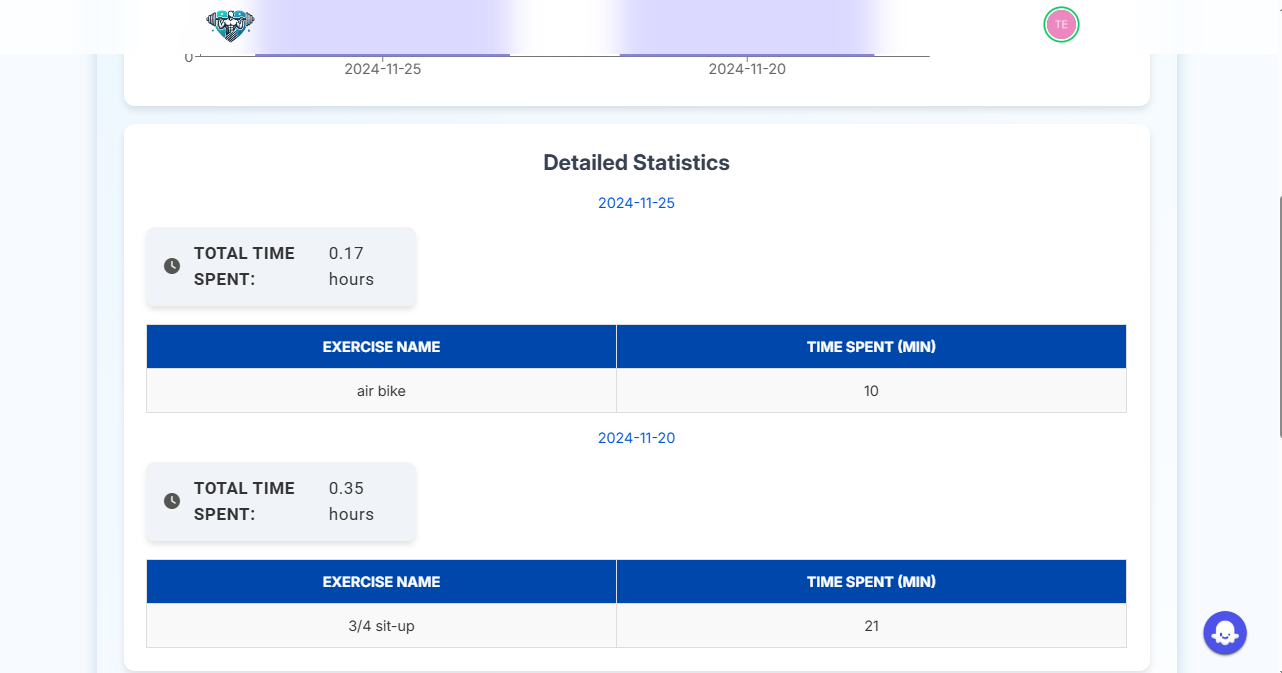
\includegraphics[width=0.86\textwidth,height=0.62\textheight,keepaspectratio]{tai_nguyen/media/image45.png}
    \caption{Giao diện thống kê kết quả tập luyện}
\end{figure}

Cửa sổ chatbot được đặt ở vị trí dễ truy cập nhưng không làm mất chức năng chính của website. Người dùng có thể hỏi nhanh về bài tập hoặc cách sử dụng hệ thống.



\begin{figure}[H]
    \centering
    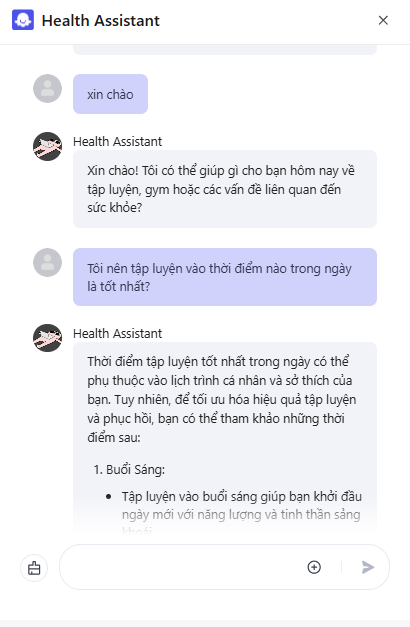
\includegraphics[width=0.86\textwidth,height=0.62\textheight,keepaspectratio]{tai_nguyen/media/image46.png}
    \caption{Giao diện trao đổi với chatbot}
\end{figure}

\section{Triển khai giao diện quản trị}

admin.jsx triển khai dashboard dành cho tài khoản có quyền quản trị. Loader kiểm tra xác thực Auth0, tìm người dùng theo email, kiểm tra cờ isAdmin và chuyển hướng về trang lỗi nếu không đủ quyền. Khi hợp lệ, admin nhận dữ liệu thống kê, danh sách người dùng và danh sách bài tập.


Giao diện quản trị có ba nhóm chính: dashboard tổng quan, quản lý người dùng và quản lý bài tập. Admin có thể sửa email, tên người dùng, quyền admin, xóa tài khoản, thêm bài tập, sửa bài tập hoặc xóa bài tập. Các thao tác này gọi đến các route update\_user, delete\_user, create\_exercise, update\_exercise và delete\_exercise.



\begin{figure}[H]
    \centering
    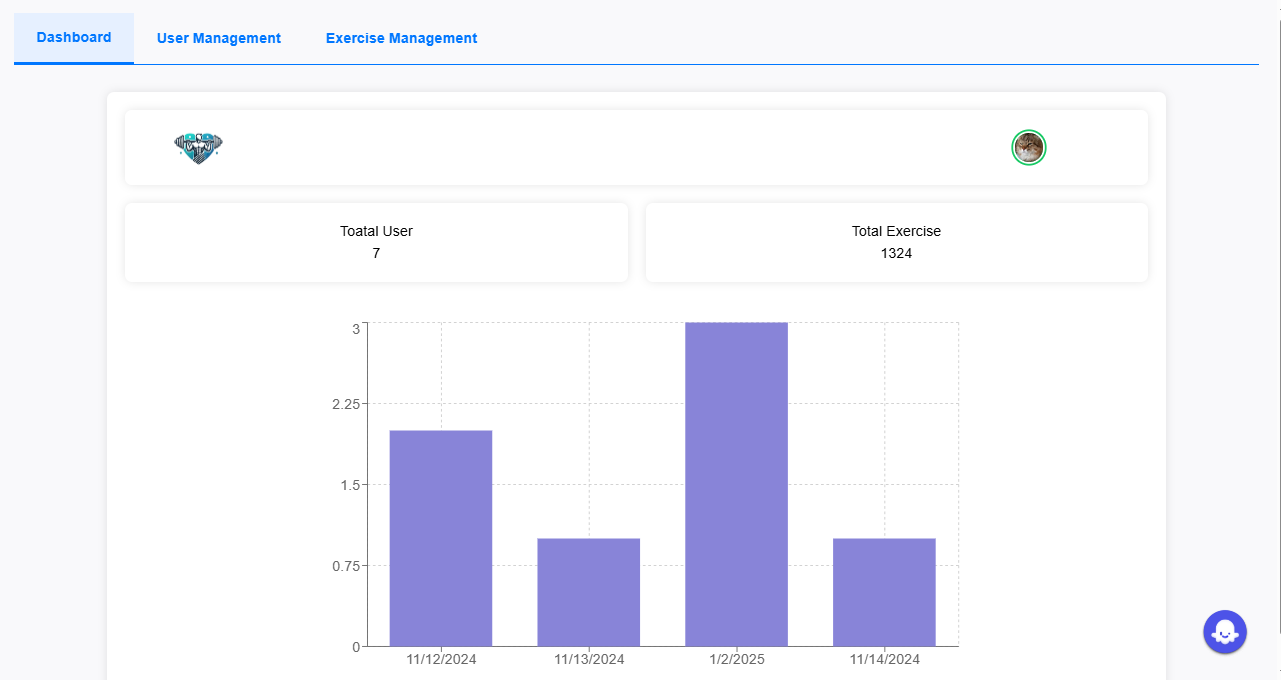
\includegraphics[width=0.86\textwidth,height=0.62\textheight,keepaspectratio]{tai_nguyen/media/image47.png}
    \caption{Giao diện tổng quan dành cho quản trị viên}
\end{figure}


\begin{figure}[H]
    \centering
    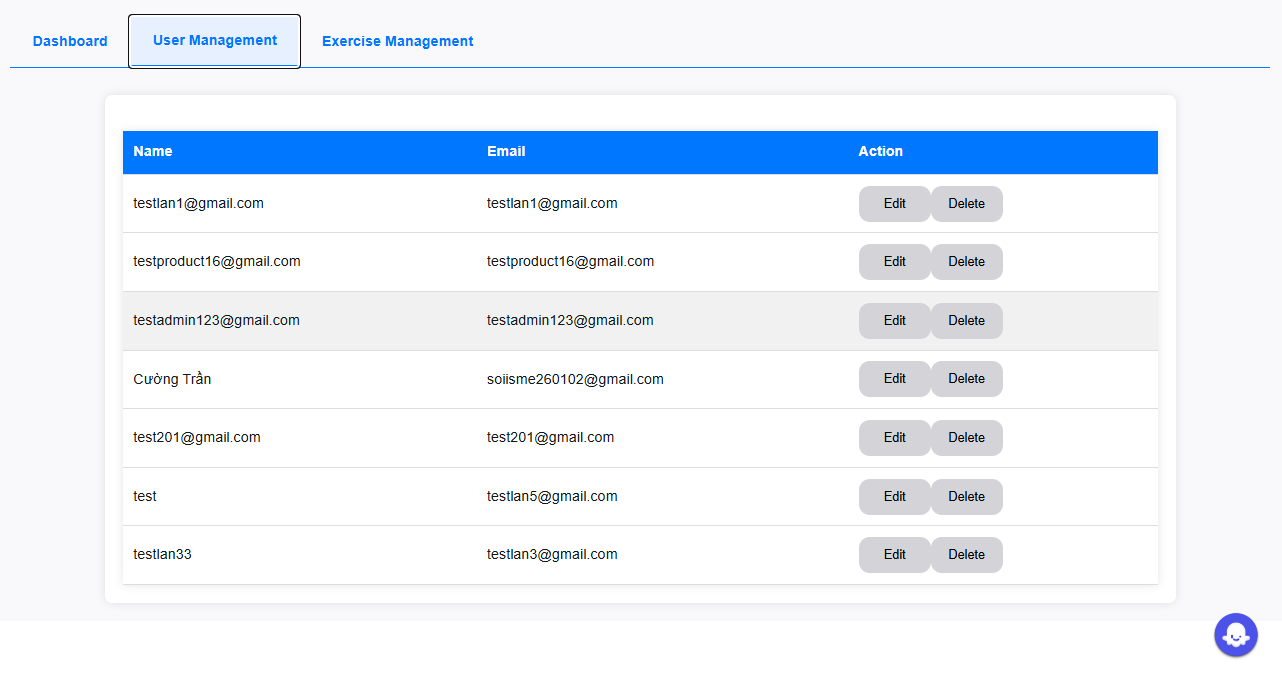
\includegraphics[width=0.86\textwidth,height=0.62\textheight,keepaspectratio]{tai_nguyen/media/image48.png}
    \caption{Giao diện quản lý tài khoản người dùng}
\end{figure}


\begin{figure}[H]
    \centering
    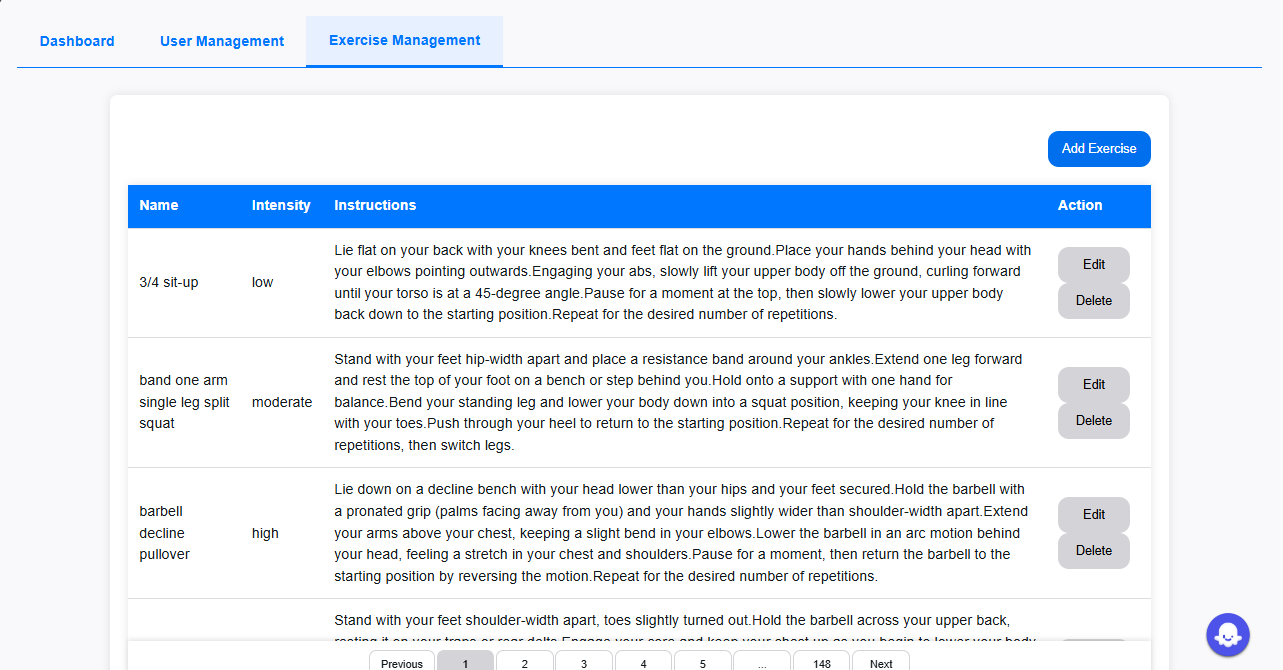
\includegraphics[width=0.86\textwidth,height=0.62\textheight,keepaspectratio]{tai_nguyen/media/image49.png}
    \caption{Giao diện quản lý dữ liệu bài tập}
\end{figure}

\section{Kiểm thử chức năng}

Kiểm thử được thực hiện theo từng luồng nghiệp vụ. Mỗi ca kiểm thử gồm điều kiện đầu vào, thao tác, kết quả mong đợi và trạng thái. Kiểm thử tập trung vào các chức năng có tác động đến dữ liệu như đăng nhập, hồ sơ sức khỏe, gợi ý, lưu kế hoạch, ghi tiến trình, thống kê và quản trị.


\begingroup
\small
\setlength{\tabcolsep}{3pt}
\renewcommand{\arraystretch}{1.25}
\begin{longtable}{|P{0.160\textwidth}|P{0.280\textwidth}|P{0.280\textwidth}|P{0.200\textwidth}|}
\caption{Kịch bản kiểm thử chức năng chính}\\
\hline
\textbf{Mã} & \textbf{Kịch bản} & \textbf{Kết quả mong đợi} & \textbf{Trạng thái} \\
\hline
\endfirsthead
\caption[]{Kịch bản kiểm thử chức năng chính (tiếp theo)}\\
\hline
\textbf{Mã} & \textbf{Kịch bản} & \textbf{Kết quả mong đợi} & \textbf{Trạng thái} \\
\hline
\endhead
TC-01 & Đăng nhập bằng tài khoản hợp lệ & Người dùng được chuyển vào hệ thống và có session userId. & Đạt \\
\hline
TC-02 & Mở trang gợi ý khi chưa có hồ sơ sức khỏe & Hệ thống trả thông báo cần cập nhật hồ sơ. & Đạt \\
\hline
TC-03 & Lưu hồ sơ sức khỏe hợp lệ & Dữ liệu được create hoặc update trong HealthStatus. & Đạt \\
\hline
TC-04 & Nhận bài tập đề xuất & Danh sách bài tập thỏa điều kiện được hiển thị. & Đạt \\
\hline
TC-05 & Lưu kế hoạch tập & WorkoutPlan tạo bản ghi theo userId và bài tập đã chọn. & Đạt \\
\hline
TC-06 & Sửa/xóa kế hoạch & Thông số được cập nhật hoặc bản ghi bị xóa. & Đạt \\
\hline
TC-07 & Lưu tiến trình từ trang chi tiết & UserProgress được tạo hoặc cập nhật. & Đạt \\
\hline
TC-08 & Xem thống kê & Biểu đồ và phản hồi được tạo từ dữ liệu tiến trình. & Đạt \\
\hline
TC-09 & Truy cập admin bằng user thường & Hệ thống chuyển hướng hoặc từ chối quyền truy cập. & Đạt \\
\hline
TC-10 & Admin thêm/sửa/xóa bài tập & Dữ liệu Exercise thay đổi đúng thao tác. & Đạt \\
\hline
\end{longtable}
\endgroup


\begin{figure}[H]
    \centering
    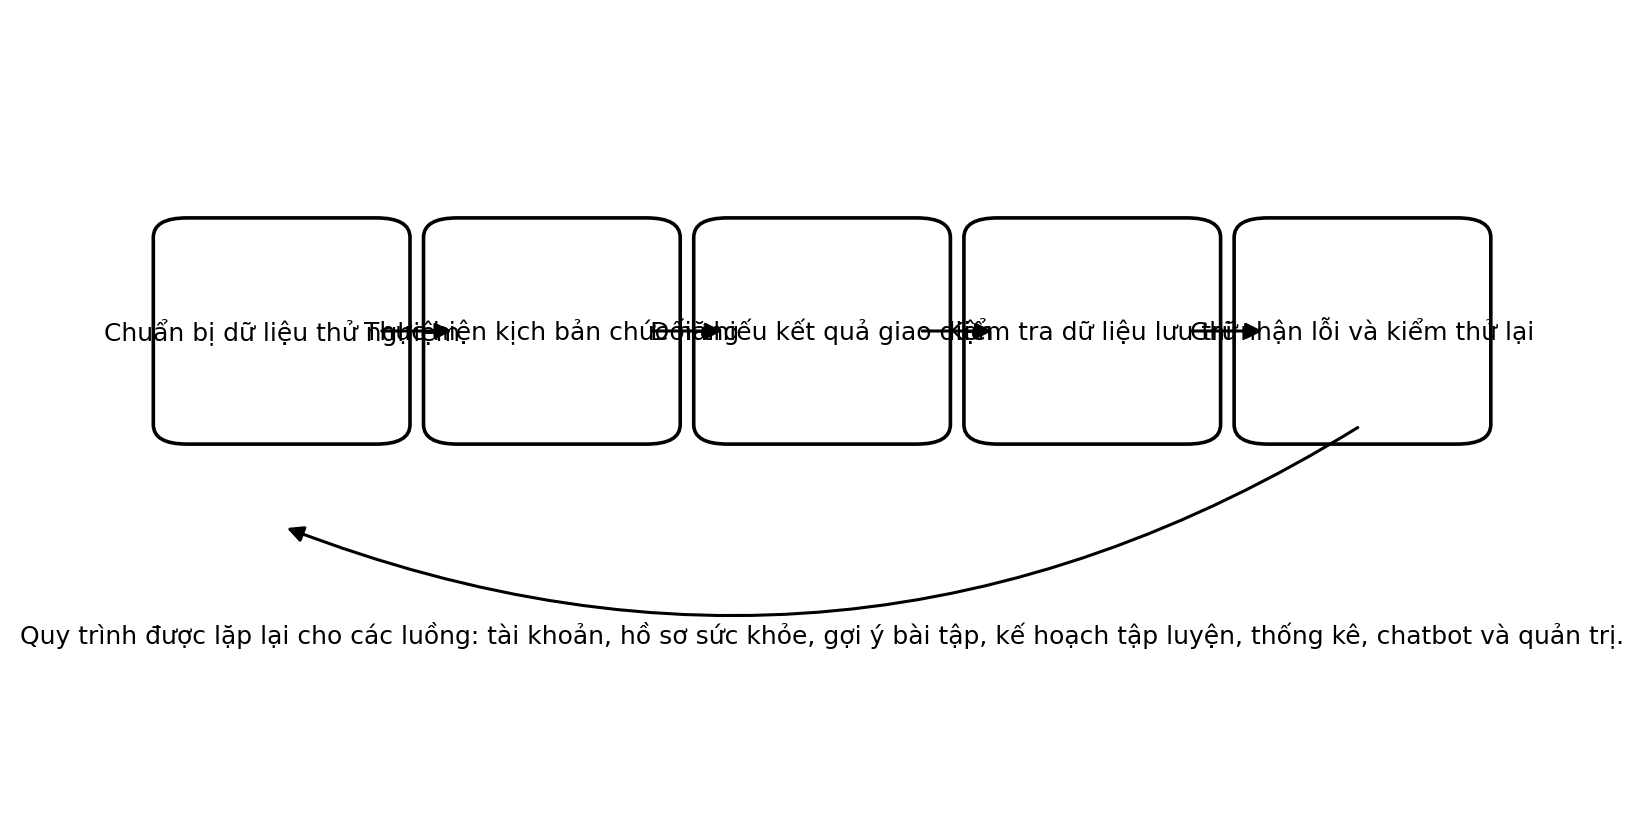
\includegraphics[width=0.86\textwidth,height=0.62\textheight,keepaspectratio]{tai_nguyen/media/image50.png}
    \caption{Quy trình kiểm thử các luồng chức năng}
\end{figure}

\section{Đánh giá bảo mật khi triển khai}

Ở mức sản phẩm thử nghiệm, hệ thống đã có xác thực Auth0 và kiểm tra session cho các route cần dữ liệu cá nhân. Tuy nhiên, khi triển khai thật cần rà soát toàn bộ secret, API key, token chatbot và khóa RapidAPI. Những giá trị này phải đặt trong biến môi trường hoặc hệ thống quản lý secret, không lưu trực tiếp trong mã nguồn.


Một số route quản trị đã kiểm tra quyền ở loader của trang admin. Tuy vậy, để an toàn hơn, các action quản trị cũng nên kiểm tra lại quyền admin trước khi thực hiện create, update hoặc delete. Đây là lớp bảo vệ cần thiết vì người dùng có thể gửi request trực tiếp mà không thông qua giao diện.


Dữ liệu sức khỏe là dữ liệu nhạy cảm ở mức cá nhân. Vì vậy, hệ thống cần giới hạn hiển thị theo userId, không cho user xem hồ sơ của người khác và chỉ đưa thông tin tối thiểu vào chatbot.


\section{Đánh giá kết quả triển khai}

\begingroup
\setlength{\tabcolsep}{3pt}
\renewcommand{\arraystretch}{1.25}
\begin{longtable}{|P{0.220\textwidth}|P{0.330\textwidth}|P{0.370\textwidth}|}
\caption{Đối chiếu kết quả triển khai với mục tiêu}\\
\hline
\textbf{Mục tiêu} & \textbf{Kết quả đạt được} & \textbf{Nhận xét} \\
\hline
\endfirsthead
\caption[]{Đối chiếu kết quả triển khai với mục tiêu (tiếp theo)}\\
\hline
\textbf{Mục tiêu} & \textbf{Kết quả đạt được} & \textbf{Nhận xét} \\
\hline
\endhead
Xác thực tài khoản & Đã cấu hình Auth0, session và tạo User nội bộ. & Đáp ứng chức năng nền tảng. \\
\hline
Hồ sơ sức khỏe & Đã có form nhập và API lưu/cập nhật. & Phục vụ trực tiếp cho gợi ý. \\
\hline
Thư viện bài tập & Đã có danh sách, tìm kiếm, phân trang và chi tiết. & Có thể mở rộng thêm bộ lọc. \\
\hline
Gợi ý cá nhân hóa & Đã lọc theo nhóm cơ, thiết bị, cường độ và sức khỏe. & Phù hợp với phạm vi rule-based. \\
\hline
Kế hoạch tập & Đã lưu, xem, sửa và xóa kế hoạch. & Đáp ứng nhu cầu theo dõi lịch. \\
\hline
Tiến trình và thống kê & Đã ghi nhận thời gian, trạng thái và tạo phản hồi. & Cần bổ sung thêm chỉ số nếu triển khai thực tế. \\
\hline
Chatbot & Đã nhúng trợ lý hội thoại vào giao diện. & Cần tiếp tục kiểm soát nội dung trả lời. \\
\hline
Quản trị & Đã có dashboard, quản lý user và bài tập. & Cần tăng kiểm tra quyền ở action. \\
\hline
\end{longtable}
\endgroup

\section{Hướng dẫn vận hành và bảo trì}

\begin{itemize}

    \item Khi chạy hệ thống ở môi trường phát triển, cần cấu hình các biến môi trường cho Auth0, session secret, database URL và các dịch vụ ngoài. Sau đó chạy migration Prisma nếu có schema, nạp dữ liệu bài tập ban đầu và kiểm tra tài khoản admin.

    \item Khi cập nhật bài tập, admin nên kiểm tra đủ các trường name, target, secondaryMuscles, bodyPart, equipment, gifUrl, difficulty, time, intensity, healthConditions và instructions. Nếu thiếu các trường này, chức năng gợi ý hoặc hiển thị chi tiết có thể bị lỗi.

    \item Khi cập nhật chatbot, cần kiểm tra nội dung huấn luyện, câu trả lời mẫu và giới hạn phạm vi. Các câu hỏi liên quan đến bệnh lý, chấn thương hoặc thuốc nên được trả lời theo hướng khuyến nghị gặp chuyên gia.

\end{itemize}

	\chapter*{KẾT LUẬN}
\addcontentsline{toc}{chapter}{KẾT LUẬN}

\section*{Kết quả đạt được}

\begin{itemize}

    \item Đề tài đã xây dựng được website tập luyện cá nhân hóa với các chức năng chính: đăng nhập, quản lý hồ sơ sức khỏe, xem thư viện bài tập, nhận gợi ý, lập kế hoạch, xem lịch tập, ghi nhận tiến trình, thống kê, chatbot hỗ trợ và trang quản trị.

    \item Mã nguồn thể hiện được đặc trưng của ứng dụng full-stack Remix: loader để nạp dữ liệu, action để xử lý form, Prisma để truy vấn cơ sở dữ liệu, Auth0 để xác thực và các component React để xây dựng giao diện.

    \item Cơ chế gợi ý bài tập đã sử dụng được dữ liệu sức khỏe và thuộc tính bài tập, trong đó nhóm cơ, thiết bị, cường độ và tình trạng sức khỏe là các tiêu chí lọc chính. Trang thống kê đã có logic đánh giá theo tuần/tháng và sinh phản hồi cá nhân hóa ở mức tham khảo.

    \item Báo cáo đã được trình bày lại theo hướng chi tiết hơn, tăng phần phân tích dựa trên mã nguồn thực tế, bổ sung ma trận route, tiêu chí kiểm thử, đánh giá bảo mật và hướng vận hành.

\end{itemize}

\section*{Hạn chế}

\begin{itemize}

    \item Cơ chế gợi ý vẫn là rule-based, chưa học từ lịch sử hành vi dài hạn hoặc phản hồi sau tập.

    \item Một số cấu hình dịch vụ trong mã nguồn thử nghiệm cần được chuyển hoàn toàn sang biến môi trường trước khi triển khai thật.

    \item Chatbot hiện chủ yếu ở dạng nhúng, chưa có pipeline kiểm soát câu trả lời riêng trong backend của hệ thống.

    \item Phần kiểm thử chủ yếu là kiểm thử thủ công theo luồng chức năng, chưa có bộ test tự động hoặc kiểm thử tải đầy đủ.

    \item Giao diện đã có responsive ở một số khu vực nhưng cần tiếp tục rà soát trên nhiều kích thước màn hình.

\end{itemize}

\section*{Hướng phát triển}

\begin{itemize}

    \item Bổ sung thuật toán khuyến nghị nâng cao dựa trên lịch sử tập luyện, mức độ hoàn thành, phản hồi sau bài tập và mục tiêu dài hạn.

    \item Tách chatbot thành một backend API có kiểm soát dữ liệu, log và giới hạn nội dung rõ ràng hơn.

    \item Tích hợp thiết bị đeo thông minh hoặc nguồn dữ liệu sức khỏe bên ngoài nếu có điều kiện triển khai thực tế.

    \item Bổ sung thông báo nhắc lịch tập, lịch tuần/tháng, đánh giá xu hướng và đề xuất phục hồi sau buổi tập.

    \item Tăng cường bảo mật bằng kiểm tra quyền ở tất cả action quản trị, ẩn secret, ghi log thao tác admin và chuẩn hóa quy trình backup dữ liệu.

\end{itemize}

	\chapter*{TÀI LIỆU THAM KHẢO}
\addcontentsline{toc}{chapter}{TÀI LIỆU THAM KHẢO}

[1]. Remix Documentation, Full Stack Web Framework for React.\par

[2]. Prisma Documentation, Prisma ORM and database access patterns.\par

[3]. Auth0 Documentation, Authentication and authorization for web applications.\par

[4]. PostgreSQL Documentation, Relational database management system.\par

[5]. NextUI Documentation, React UI components.\par

[6]. Recharts Documentation, Charting library for React.\par

[7]. Dify/Coze chatbot embedding documentation and project integration notes.\par

[8]. Mã nguồn project Web thể dục do sinh viên cung cấp: root.jsx, auth.server.js, db.server.js và các route trong thư mục app/routes.\par

	
	% Appendices
	\clearpage
	\addcontentsline{toc}{chapter}{PHỤ LỤC}
	\appendix
	\renewcommand{\chaptername}{Phụ lục}
	\phulucchapter{CÂU HỎI KHẢO SÁT ĐỀ XUẤT}

\begin{itemize}

    \item Anh/chị thường tập luyện trong khoảng thời gian nào trong ngày?

    \item Anh/chị gặp khó khăn gì khi tự tập luyện tại nhà?

    \item Anh/chị có sẵn sàng cung cấp cân nặng, chiều cao và mục tiêu tập luyện để nhận gợi ý không?

    \item Anh/chị có thiết bị hỗ trợ nào như tạ tay, dây kháng lực hoặc thảm tập không?

    \item Anh/chị muốn hệ thống gợi ý bài tập theo mục tiêu, nhóm cơ hay thời gian?

    \item Anh/chị có cần chức năng lưu lịch tập theo ngày không?

    \item Anh/chị muốn xem thống kê theo tuần, tháng hay từng bài tập?

    \item Anh/chị có cần chatbot hướng dẫn cách dùng website hoặc giải thích bài tập không?

    \item Anh/chị quan tâm nhất đến yếu tố nào: dễ dùng, cá nhân hóa, bài tập đa dạng hay thống kê?

    \item Anh/chị mong muốn website cải thiện thêm chức năng nào trong tương lai?

\end{itemize}

\phulucchapter{MẪU DỮ LIỆU BÀI TẬP SAU CHUẨN HÓA}

\begingroup
\setlength{\tabcolsep}{3pt}
\renewcommand{\arraystretch}{1.25}
\begin{longtable}{|P{0.220\textwidth}|P{0.330\textwidth}|P{0.370\textwidth}|}
\caption{Trường dữ liệu bài tập mẫu}\\
\hline
\textbf{Trường} & \textbf{Kiểu dữ liệu} & \textbf{Mô tả} \\
\hline
\endfirsthead
\caption[]{Trường dữ liệu bài tập mẫu (tiếp theo)}\\
\hline
\textbf{Trường} & \textbf{Kiểu dữ liệu} & \textbf{Mô tả} \\
\hline
\endhead
id & String & Mã định danh bài tập. \\
\hline
name & String & Tên bài tập. \\
\hline
target & String & Nhóm cơ chính. \\
\hline
secondaryMuscles & Array<String> & Danh sách nhóm cơ phụ. \\
\hline
bodyPart & String & Bộ phận cơ thể liên quan. \\
\hline
equipment & String & Thiết bị cần sử dụng. \\
\hline
gifUrl & String & Đường dẫn ảnh động hoặc hình minh họa. \\
\hline
difficulty & String & easy, medium hoặc hard. \\
\hline
time & Number & Thời lượng ước lượng theo phút. \\
\hline
intensity & String & low, moderate hoặc high. \\
\hline
healthConditions & Array<String> & Nhóm sức khỏe phù hợp. \\
\hline
instructions & Array<String> & Các bước hướng dẫn thực hiện. \\
\hline
\end{longtable}
\endgroup

\phulucchapter{CHECKLIST NGHIỆM THU CHỨC NĂNG}

\begingroup
\setlength{\tabcolsep}{3pt}
\renewcommand{\arraystretch}{1.25}
\begin{longtable}{|P{0.220\textwidth}|P{0.330\textwidth}|P{0.370\textwidth}|}
\caption{Checklist nghiệm thu}\\
\hline
\textbf{Nhóm} & \textbf{Mục kiểm tra} & \textbf{Kết quả} \\
\hline
\endfirsthead
\caption[]{Checklist nghiệm thu (tiếp theo)}\\
\hline
\textbf{Nhóm} & \textbf{Mục kiểm tra} & \textbf{Kết quả} \\
\hline
\endhead
Auth & Đăng nhập thành công và tạo session. & Đạt \\
\hline
User & Tạo mới User khi tài khoản chưa tồn tại. & Đạt \\
\hline
Health & Lưu/cập nhật hồ sơ sức khỏe. & Đạt \\
\hline
Exercise & Tìm kiếm và phân trang danh sách bài tập. & Đạt \\
\hline
Recommendation & Lọc bài tập theo hồ sơ sức khỏe. & Đạt \\
\hline
Plan & Lưu kế hoạch và hiển thị theo ngày. & Đạt \\
\hline
Progress & Lưu thời gian tập và trạng thái hoàn thành. & Đạt \\
\hline
Stats & Tạo biểu đồ và phản hồi cá nhân hóa. & Đạt \\
\hline
Admin & Quản lý người dùng và bài tập. & Đạt \\
\hline
Chatbot & Hiển thị cửa sổ chatbot trên website. & Đạt \\
\hline
\end{longtable}
\endgroup

\phulucchapter{GIẢ MÃ THUẬT TOÁN GỢI Ý BÀI TẬP}

\begin{itemize}

    \item Input: userHealthStatus gồm targetMuscleGroups, equipmentPreference, intensityPreference, condition.

    \item Bước 1: Đọc hồ sơ sức khỏe của người dùng từ cơ sở dữ liệu.

    \item Bước 2: Tạo danh sách điều kiện lọc. Điều kiện rỗng sẽ bị loại bỏ.

    \item Bước 3: Truy vấn bảng Exercise với AND các điều kiện còn lại.

    \item Bước 4: Xóa danh sách Workout cũ của người dùng để tránh dữ liệu lỗi thời.

    \item Bước 5: Tạo bản ghi Workout mới cho từng bài tập được đề xuất.

    \item Output: danh sách bài tập phù hợp để hiển thị trên giao diện.

\end{itemize}

\phulucchapter{MA TRẬN MÃ NGUỒN VÀ CHỨC NĂNG}

\begingroup
\setlength{\tabcolsep}{3pt}
\renewcommand{\arraystretch}{1.25}
\begin{longtable}{|P{0.220\textwidth}|P{0.330\textwidth}|P{0.370\textwidth}|}
\caption{Ma trận mã nguồn trọng tâm}\\
\hline
\textbf{Nhóm} & \textbf{File} & \textbf{Nội dung cần bảo trì} \\
\hline
\endfirsthead
\caption[]{Ma trận mã nguồn trọng tâm (tiếp theo)}\\
\hline
\textbf{Nhóm} & \textbf{File} & \textbf{Nội dung cần bảo trì} \\
\hline
\endhead
Nền tảng & root.jsx & Layout, provider, chatbot, script dịch ngôn ngữ. \\
\hline
Xác thực & auth.server.js & Cookie session, Authenticator, Auth0Strategy. \\
\hline
Dữ liệu & db.server.js & PrismaClient và kết nối cơ sở dữ liệu. \\
\hline
Trang chủ & home.jsx & Tìm kiếm, phân trang, hiển thị bài tập. \\
\hline
Hồ sơ & HealthStatus.jsx & Form sức khỏe, chọn thiết bị, chọn nhóm cơ. \\
\hline
Hồ sơ API & healthstatusapi.jsx & Create/update HealthStatus. \\
\hline
Gợi ý & Recommended.workout.jsx & Lọc bài tập theo hồ sơ. \\
\hline
Kế hoạch & WorkoutPlan.jsx, Workout.jsx & Lập và xem lịch tập. \\
\hline
Tiến trình & userprogressapi.jsx & Lưu trạng thái và thời gian tập. \\
\hline
Thống kê & Stats.jsx & Đánh giá tuần/tháng, biểu đồ, phản hồi. \\
\hline
Quản trị & admin.jsx & Dashboard, quản lý user và bài tập. \\
\hline
Chatbot & chatbotapi2.jsx & Nhúng chatbot và tùy biến giao diện. \\
\hline
\end{longtable}
\endgroup

\phulucchapter{KỊCH BẢN KIỂM THỬ CHI TIẾT}

Phụ lục này mở rộng phần kiểm thử bằng cách mô tả rõ hơn dữ liệu đầu vào và tiêu chí quan sát. Các ca kiểm thử được xây dựng theo luồng người dùng thực tế, từ xác thực đến cập nhật hồ sơ, nhận gợi ý, lập kế hoạch, lưu tiến trình và quản trị dữ liệu. Khi triển khai lại trên môi trường khác, người kiểm thử có thể dùng bảng này như checklist nghiệm thu tối thiểu.


\begingroup
\small
\setlength{\tabcolsep}{3pt}
\renewcommand{\arraystretch}{1.25}
\begin{longtable}{|P{0.160\textwidth}|P{0.280\textwidth}|P{0.280\textwidth}|P{0.200\textwidth}|}
\caption{Kịch bản kiểm thử chi tiết theo luồng người dùng}\\
\hline
\textbf{Mã ca} & \textbf{Điều kiện đầu vào} & \textbf{Thao tác kiểm thử} & \textbf{Kết quả cần quan sát} \\
\hline
\endfirsthead
\caption[]{Kịch bản kiểm thử chi tiết theo luồng người dùng (tiếp theo)}\\
\hline
\textbf{Mã ca} & \textbf{Điều kiện đầu vào} & \textbf{Thao tác kiểm thử} & \textbf{Kết quả cần quan sát} \\
\hline
\endhead
AUTH-01 & Chưa đăng nhập & Mở trang cần xác thực & Hệ thống yêu cầu đăng nhập hoặc trả lỗi 401. \\
\hline
AUTH-02 & Tài khoản Auth0 hợp lệ & Đăng nhập và quay về callback & User được tạo nếu chưa tồn tại, session có userId. \\
\hline
AUTH-03 & Tài khoản thường & Truy cập /admin & Bị chuyển sang trang 404 hoặc bị từ chối quyền. \\
\hline
HEALTH-01 & Đã đăng nhập & Nhập đủ hồ sơ sức khỏe và lưu & Bản ghi HealthStatus được tạo mới. \\
\hline
HEALTH-02 & Đã có HealthStatus & Thay đổi mục tiêu, cường độ và lưu & Bản ghi cũ được cập nhật, không tạo trùng. \\
\hline
HEALTH-03 & Chọn cường độ moderate & Gọi equipmentapi & Danh sách thiết bị phù hợp được trả về. \\
\hline
HEALTH-04 & Đã chọn thiết bị & Gọi musclesapi & Danh sách nhóm cơ phù hợp với thiết bị và cường độ. \\
\hline
EXERCISE-01 & Có dữ liệu Exercise & Tìm kiếm theo tên bài tập & Danh sách lọc theo từ khóa, không lỗi khi rỗng. \\
\hline
EXERCISE-02 & Chọn bài tập bất kỳ & Mở trang chi tiết & Thông tin target, equipment, gifUrl, instructions hiển thị. \\
\hline
REC-01 & Có HealthStatus hợp lệ & Mở Recommended workout & Danh sách gợi ý đúng cường độ, thiết bị, nhóm cơ. \\
\hline
REC-02 & Thay đổi hồ sơ & Mở lại Recommended workout & Workout cũ bị xóa và danh sách mới được tạo. \\
\hline
PLAN-01 & Chọn nhiều bài tập & Lưu kế hoạch qua Workoutplanapi & Mỗi bài tạo một bản ghi WorkoutPlan. \\
\hline
PLAN-02 & Có kế hoạch đã lưu & Mở Workout & Các bài được nhóm theo ngày hoặc hiển thị đúng thông số. \\
\hline
PLAN-03 & Có bài trong kế hoạch & Sửa time, sets, reps & Dữ liệu được cập nhật qua editworkoutapi. \\
\hline
PLAN-04 & Có bài trong kế hoạch & Xóa bài tập khỏi lịch & Bản ghi WorkoutPlan bị xóa qua deleteapi. \\
\hline
PROG-01 & Đang ở ExerciseDetail & Bấm Start, Pause, Save & Thời gian tập được gửi đến userprogressapi. \\
\hline
PROG-02 & Bài tập đã có progress & Lưu lại bài đó & Bản ghi UserProgress được update thay vì tạo trùng. \\
\hline
STAT-01 & Có dữ liệu tiến trình & Mở Stats & Biểu đồ, chỉ số và feedback được hiển thị. \\
\hline
ADMIN-01 & Tài khoản admin & Mở tab User Management & Danh sách user hiển thị, sửa/xóa hoạt động. \\
\hline
ADMIN-02 & Tài khoản admin & Thêm/sửa/xóa Exercise & Dữ liệu bài tập thay đổi và không làm lỗi gợi ý. \\
\hline
\end{longtable}
\endgroup

\phulucchapter{QUY TẮC RÀ SOÁT MÃ NGUỒN TRƯỚC KHI TRIỂN KHAI}

Khi chuyển từ môi trường làm đồ án sang môi trường triển khai thật, mã nguồn cần được rà soát theo các nhóm sau. Nội dung này được bổ sung để báo cáo thể hiện rõ tính thực tế của quá trình phát triển phần mềm, đồng thời tránh đưa các cấu hình thử nghiệm vào môi trường vận hành.


\section{Rà soát cấu hình và biến môi trường}

\begin{itemize}

    \item Toàn bộ domain Auth0, client id, client secret, callback URL, logout URL và session secret phải lấy từ biến môi trường thay vì ghi cố định trong file mã nguồn.

    \item Các token chatbot, khóa RapidAPI hoặc khóa dịch vụ ngoài cần được đặt ở server/secret manager. Giao diện chỉ gọi backend nội bộ, không tự mang khóa bí mật.

    \item Cấu hình callback cần tách rõ localhost, staging và production để tránh lỗi đăng nhập sau khi deploy.

    \item File .env thật không được nộp kèm báo cáo hoặc đưa lên kho Git công khai. Nếu cần minh họa, chỉ dùng .env.example với giá trị giả.

\end{itemize}

\section{Rà soát quyền truy cập}

\begin{itemize}

    \item Mỗi action có tác động dữ liệu như create\_exercise, update\_exercise, delete\_exercise, update\_user và delete\_user nên kiểm tra lại quyền admin ở phía server.

    \item Các route người dùng như healthstatusapi, Workoutplanapi và userprogressapi cần luôn lấy userId từ session, không tin vào userId gửi từ form.

    \item Khi xóa user, cần cân nhắc xóa hoặc vô hiệu hóa dữ liệu liên quan như HealthStatus, WorkoutPlan và UserProgress để tránh bản ghi mồ côi.

    \item Khi sửa dữ liệu bài tập, cần kiểm tra định dạng mảng secondaryMuscles, healthConditions và instructions trước khi lưu.

\end{itemize}

\section{Rà soát dữ liệu và trải nghiệm}

\begin{itemize}

    \item Thêm thông báo rõ ràng khi chưa có hồ sơ sức khỏe nhưng người dùng mở trang gợi ý.

    \item Kiểm tra ảnh gifUrl không hỏng trước khi lưu bài tập mới.

    \item Thêm trạng thái loading cho các thao tác cần chờ như lưu hồ sơ, tạo kế hoạch, tải video và gọi chatbot.

    \item Đồng bộ cách dùng chữ hoa/thường cho model Prisma như Exercise/exercise hoặc User/user để tránh lỗi khi chuyển môi trường.

    \item Chuẩn hóa route có dấu chấm như Recommended.workout.jsx để bảo đảm đường dẫn đúng mong muốn của Remix.

\end{itemize}

\phulucchapter{PHÂN TÍCH CÁC ĐIỂM CẦN HOÀN THIỆN TỪ MÃ NGUỒN}

Phụ lục này không nhằm phê bình sản phẩm mà dùng để chứng minh quá trình đọc và đối chiếu mã nguồn. Một báo cáo đồ án tốt nên chỉ ra được phần đã làm, phần còn hạn chế và phương án hoàn thiện. Các nhận xét dưới đây được trình bày theo hướng kỹ thuật, tránh nêu thông tin nhạy cảm như khóa API hoặc token thật.


\begingroup
\setlength{\tabcolsep}{3pt}
\renewcommand{\arraystretch}{1.25}
\begin{longtable}{|P{0.220\textwidth}|P{0.330\textwidth}|P{0.370\textwidth}|}
\caption{Điểm cần hoàn thiện và phương án đề xuất}\\
\hline
\textbf{Nhóm} & \textbf{Hiện trạng quan sát} & \textbf{Đề xuất hoàn thiện} \\
\hline
\endfirsthead
\caption[]{Điểm cần hoàn thiện và phương án đề xuất (tiếp theo)}\\
\hline
\textbf{Nhóm} & \textbf{Hiện trạng quan sát} & \textbf{Đề xuất hoàn thiện} \\
\hline
\endhead
Xác thực & Một số callback/redirect đang dùng địa chỉ localhost. & Tách URL theo biến môi trường AUTH0\_CALLBACK\_URL, AUTH0\_RETURN\_TO\_URL. \\
\hline
Đăng xuất & auth.logout.jsx có đoạn tham chiếu biến Auth0 domain/clientId/returnTo cần cấu hình đầy đủ. & Đọc biến từ process.env và kiểm thử logout Auth0 end-to-end. \\
\hline
Bảo mật secret & Một số khóa hoặc token thử nghiệm xuất hiện trong code tích hợp ngoài. & Đưa vào .env, không đưa vào repo, tạo .env.example để minh họa. \\
\hline
Phân quyền admin & Trang admin có kiểm tra quyền ở loader, nhưng các action CRUD nên kiểm tra lại. & Viết hàm requireAdmin(request) dùng chung cho action quản trị. \\
\hline
Dữ liệu bài tập & Các trường mảng được nhập dưới dạng chuỗi rồi split bằng dấu phẩy. & Thêm hướng dẫn nhập, validate rỗng và trim dữ liệu trước khi lưu. \\
\hline
Gợi ý bài tập & Điều kiện lọc đang dựa trên target, equipment, intensity và condition. & Bổ sung thứ tự ưu tiên theo mục tiêu fitnessGoals và available\_time. \\
\hline
Thống kê & Feedback đã có nhưng còn phụ thuộc dữ liệu UserProgress. & Thêm thông báo khi dữ liệu chưa đủ, thêm chỉ số streak hoặc số ngày duy trì. \\
\hline
Chatbot & Chatbot nhúng thuận tiện nhưng backend chưa kiểm soát sâu câu trả lời. & Tạo lớp API nội bộ nếu cần lưu log, giới hạn nội dung và quản lý nguồn tri thức. \\
\hline
Video liên quan & Trang chi tiết gọi API video ngoài. & Ẩn khóa, thêm fallback khi API lỗi hoặc không có video. \\
\hline
Kiểm thử & Chủ yếu kiểm thử thủ công. & Bổ sung unit test cho hàm tính difficulty, time, intensity, healthConditions. \\
\hline
\end{longtable}
\endgroup

Những điểm trên cũng là hướng phát triển hợp lý sau khi hoàn thành phiên bản đồ án. Nếu được bổ sung, hệ thống sẽ an toàn hơn khi deploy, dễ bảo trì hơn khi mở rộng dữ liệu và có khả năng đánh giá chất lượng cá nhân hóa tốt hơn.


	
	% Supervisor comments
	\clearpage
	\chapter*{NHẬN XÉT CỦA GIÁO VIÊN HƯỚNG DẪN}
	\addcontentsline{toc}{chapter}{NHẬN XÉT CỦA GIÁO VIÊN HƯỚNG DẪN}
	\vspace{0.5cm}
\noindent\textbf{Đánh giá nội dung và kết quả thực hiện:}

\vspace{0.4cm}
\noindent\dotfill

\vspace{0.4cm}
\noindent\dotfill

\vspace{0.4cm}
\noindent\dotfill

\vspace{0.8cm}
\begin{flushright}
\begin{minipage}{0.50\textwidth}
\centering
Thái Nguyên, ngày \ldots{} tháng \ldots{} năm 2026\\[0.2cm]
\textbf{Giảng viên hướng dẫn}\\[2.0cm]
\textbf{T.S Tô Hữu Nguyên}
\end{minipage}
\end{flushright}

	
\end{document}